\documentclass[12pt]{article}

\usepackage[utf8]{inputenc}
\usepackage[T1]{fontenc}
\usepackage{lmodern}
\usepackage{graphics}
\usepackage{graphicx}
\usepackage[french]{babel}
\usepackage{fullpage}
\usepackage{float}
\usepackage{verbatim}
\usepackage[stable]{footmisc} 
\usepackage{perpage}
\usepackage{ulem}
\usepackage{caption}
\usepackage{hyperref}
\usepackage{longtable}
\MakePerPage{footnote}
\usepackage{wrapfig,blindtext}
\renewcommand{\arraystretch}{1.3}% marges tableaux

\begin{document}
	
\thispagestyle{empty}
\begin{center}
\begin{LARGE}
\begin{center}
	\textbf{GF2 - Méthodes d’acquisition et données de courantologie}
\end{center}
\end{LARGE}
\end{center}

\section{Matériel et méthodes}
L'ADCP \textit{(Acoustic Current Doppler Profiler)} et l'Aquadopp sont des courantomètres acoustiques à effet Doppler composés, respectivement, de 4 et 3 transducteurs piézoélectriques pour la transmission et la réception des signaux acoustiques, ainsi que d’une partie électronique/informatique assurant la génération et l’acquisition des signaux. Le signal acoustique émis par le capteur à une fréquence donnée se propage dans l’eau et est rétrodiffusé par les particules en suspension. Ces signaux rétrodiffusés sont reçus aux capteurs puis traités.\\
\indent On part du principe que les particules en suspension qui renvoient les signaux suivent la masse d’eau à la même vitesse que cette dernière : on calcule la vitesse de ces particules et donc du courant.\\
\indent Pour l'ADCP, il faut également connaître la vitesse, le positionnement GPS, etc. du navire pour estimer ces courants dans le repère. Ci-dessus, le cas d'un ADCP de coque comme sur le Téthys II :

\begin{figure}[!ht]
	\begin{center}
		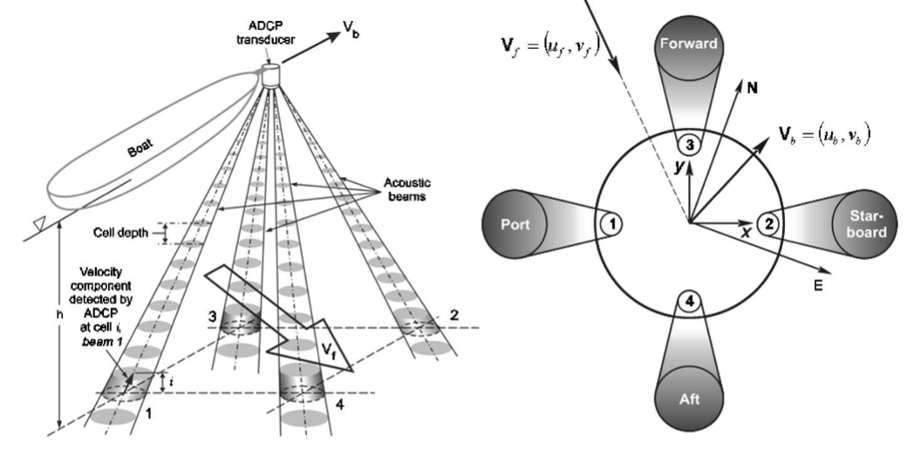
\includegraphics[width=0.8\textwidth]{adcp.png}
		\caption{Fonctionnement de l'ADCP de coque du Téthys II.}
	\end{center}
\end{figure}

\section{Aquadopp}
Modification pour test Git sisi\\
Deuxième Test on va voir 
%%%%%%%%%%%%%%%%
Les mesures prises par l'Aquadopp nous renseignent sur différents paramètres du courant sur toute la hauteur de la colonne d'eau. La direction du courant (en $^{\circ}$N), son intensité générale et son intensité selon les composantes Nord-Sud et Est-Ouest. Les informations de profondeur et de température auxquelles l'appareil est immergé sont également fournies.

\subsection{Journée du 17 mars 2021}
L'Aquadopp a été placé successivement sur les deux bords externes de la zone : voir les effets de seiches (figure 2).

\subsubsection{Emplacement 1}
Pour le premier emplacement, l'Aquadopp a été immergé à 14h30 vers 4,6 $m$ de profondeur avant d'être déclenché pour les mesures de courant de 15h20 à 16h10.
	
	\begin{figure}[!ht]
		\begin{center}
			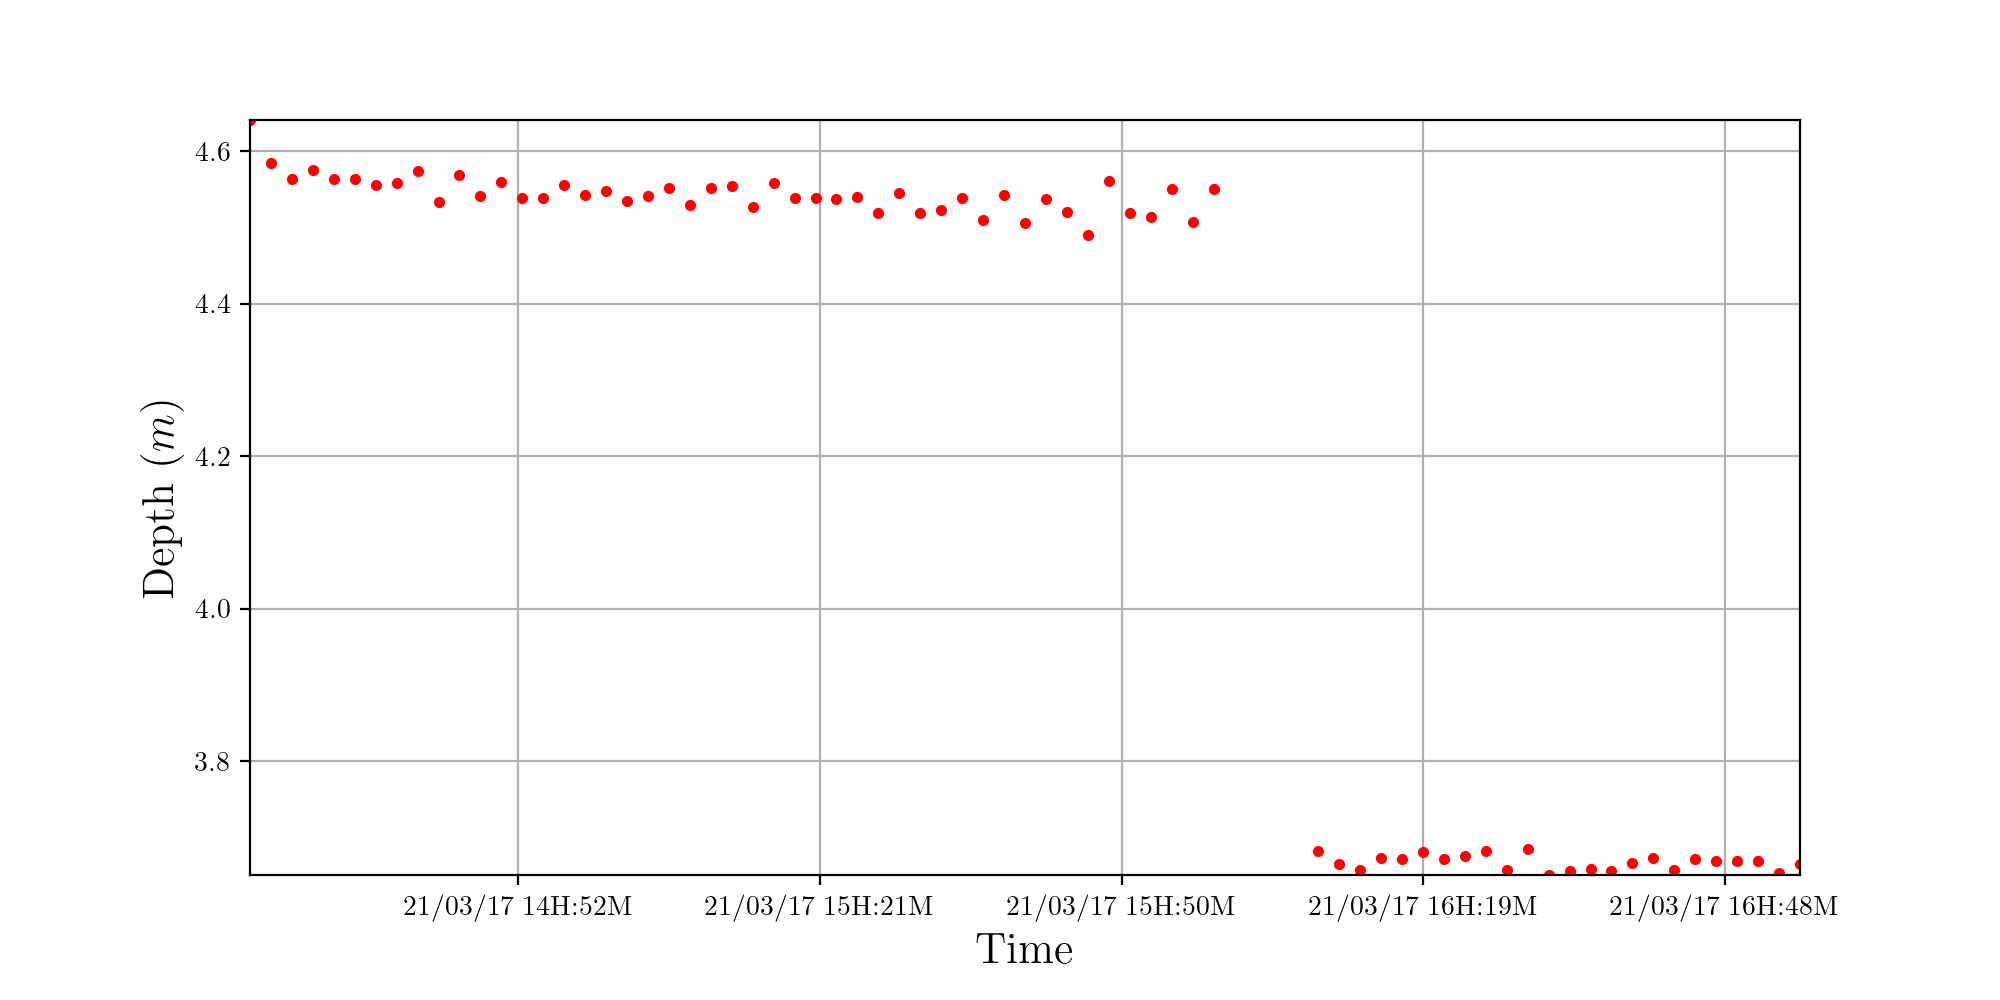
\includegraphics[width=0.8\textwidth]{1703F03depth.png}
			\caption{Profondeur mesurée d'immersion de l'Aquadopp ($m$).}
		\end{center}
	\end{figure}

\subsubsection{Emplacement 2}
	Immersion de 16h10 à 16h50 à 3,7 $m$ de profondeur.
	
\subsubsection{Résultats}
\begin{figure}[!ht]
	\begin{center}
		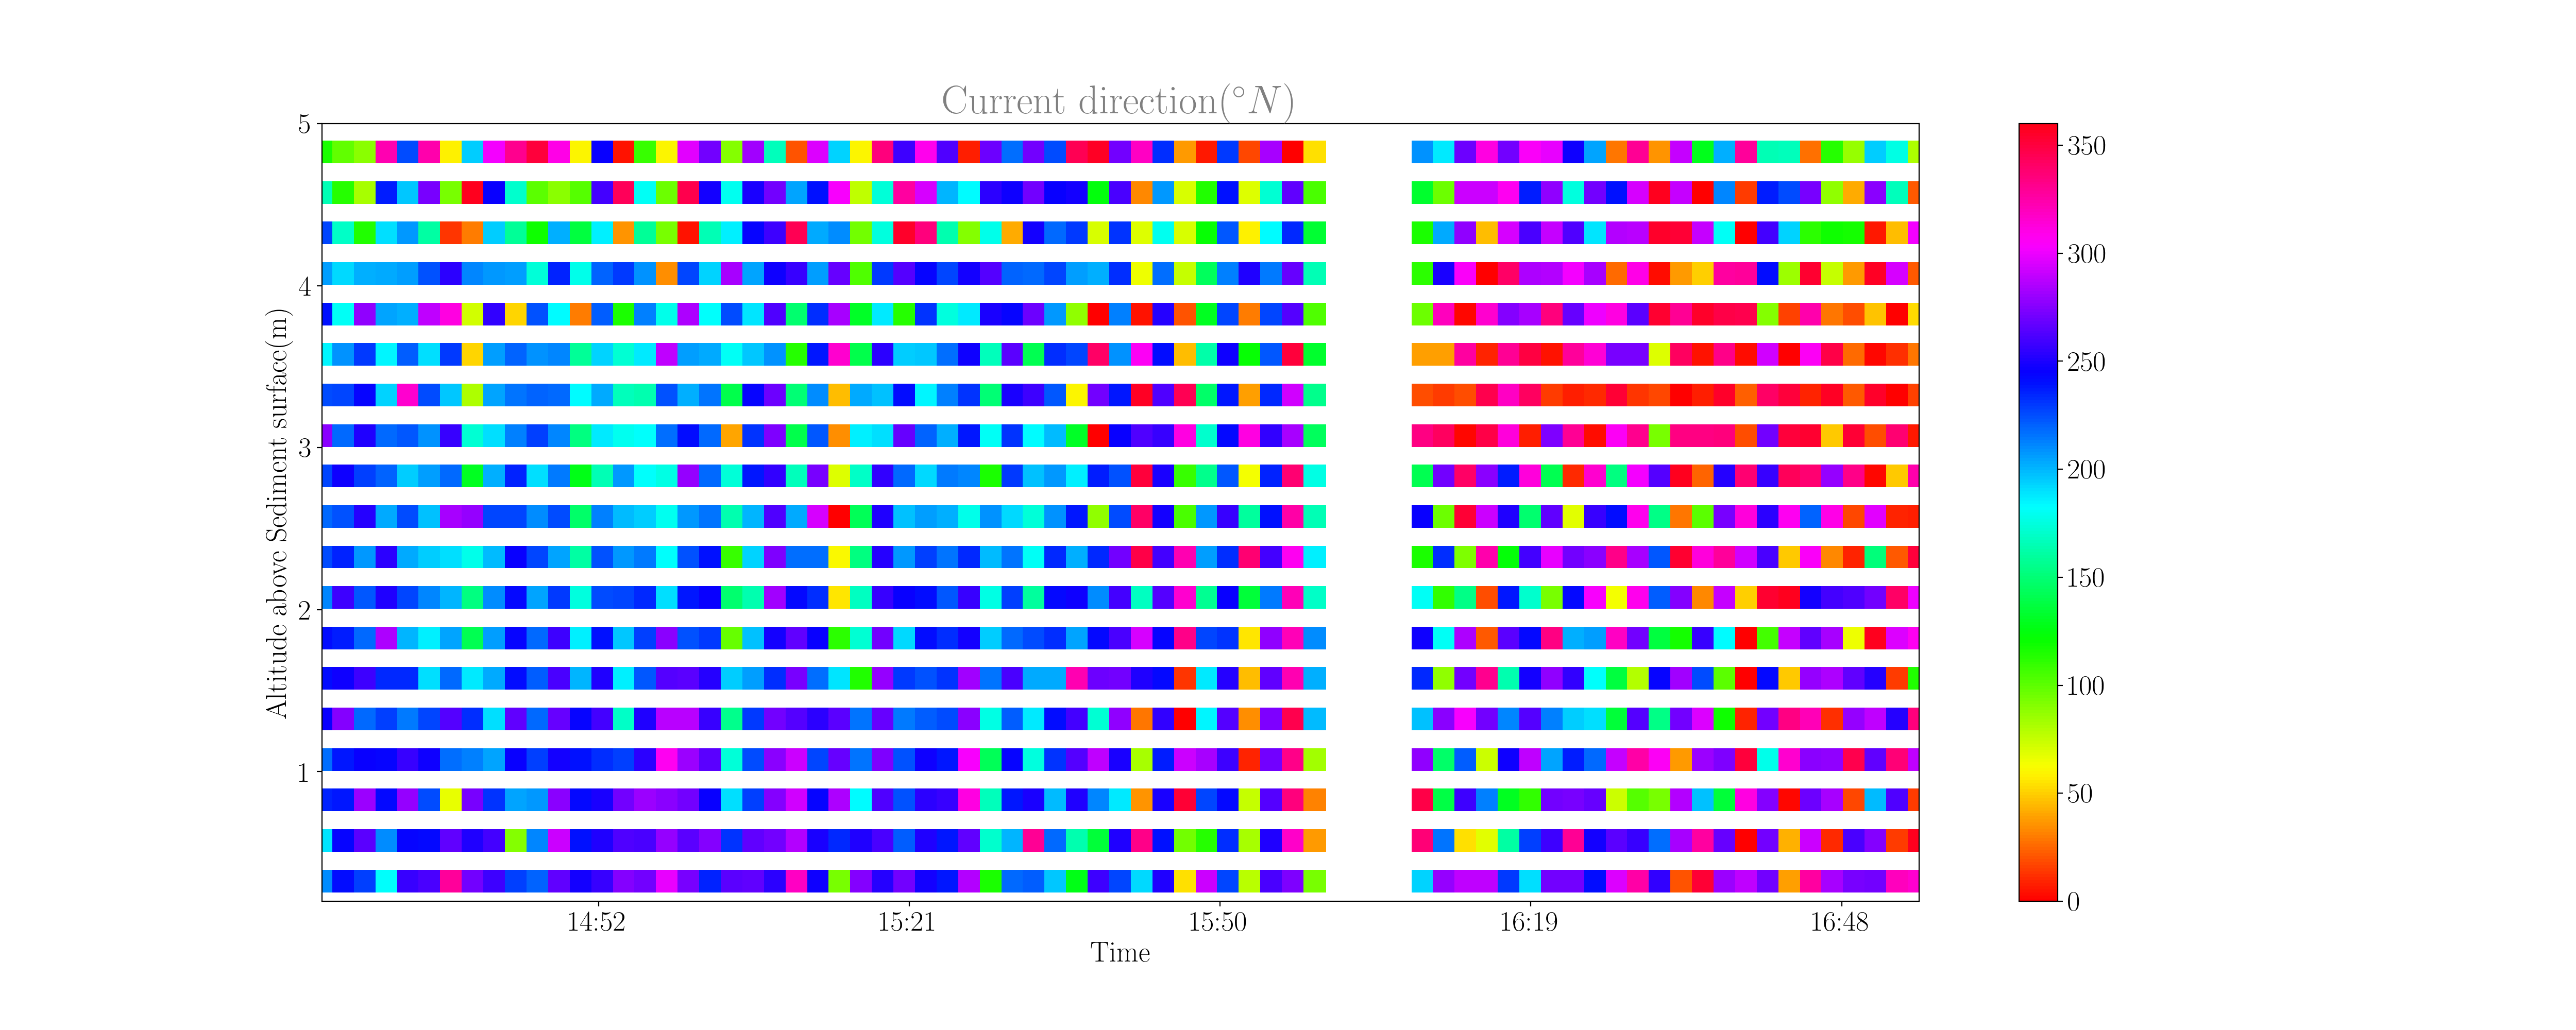
\includegraphics[width=0.8\textwidth]{1703F03scatterdirection.png}
		\caption{Direction du courant de 14h30 à 16h50 ($^{\circ}$N).}
	\end{center}
\end{figure}
\textbf{COMMENTAIRE FIGURE 3} Pour le premier emplacement, la direction du courant peut être séparée en deux temps : il varie principalement entre 200°N et 250°N pour les premières 20 minutes avant de tourner entre 300°N et 350°N.\\
\indent Pour le second emplacement, la direction du courant à la surface (entre 3 et 4 m sur la figure 3) se situe entre 300°N et 350°N. En profondeur, le courant reste relativement orienté Nord avec des valeurs comprises entre 150°N et 350°N. \textbf{FIN COM FIGURE 3} \\
	
\begin{figure}[!ht]
	\begin{center}
		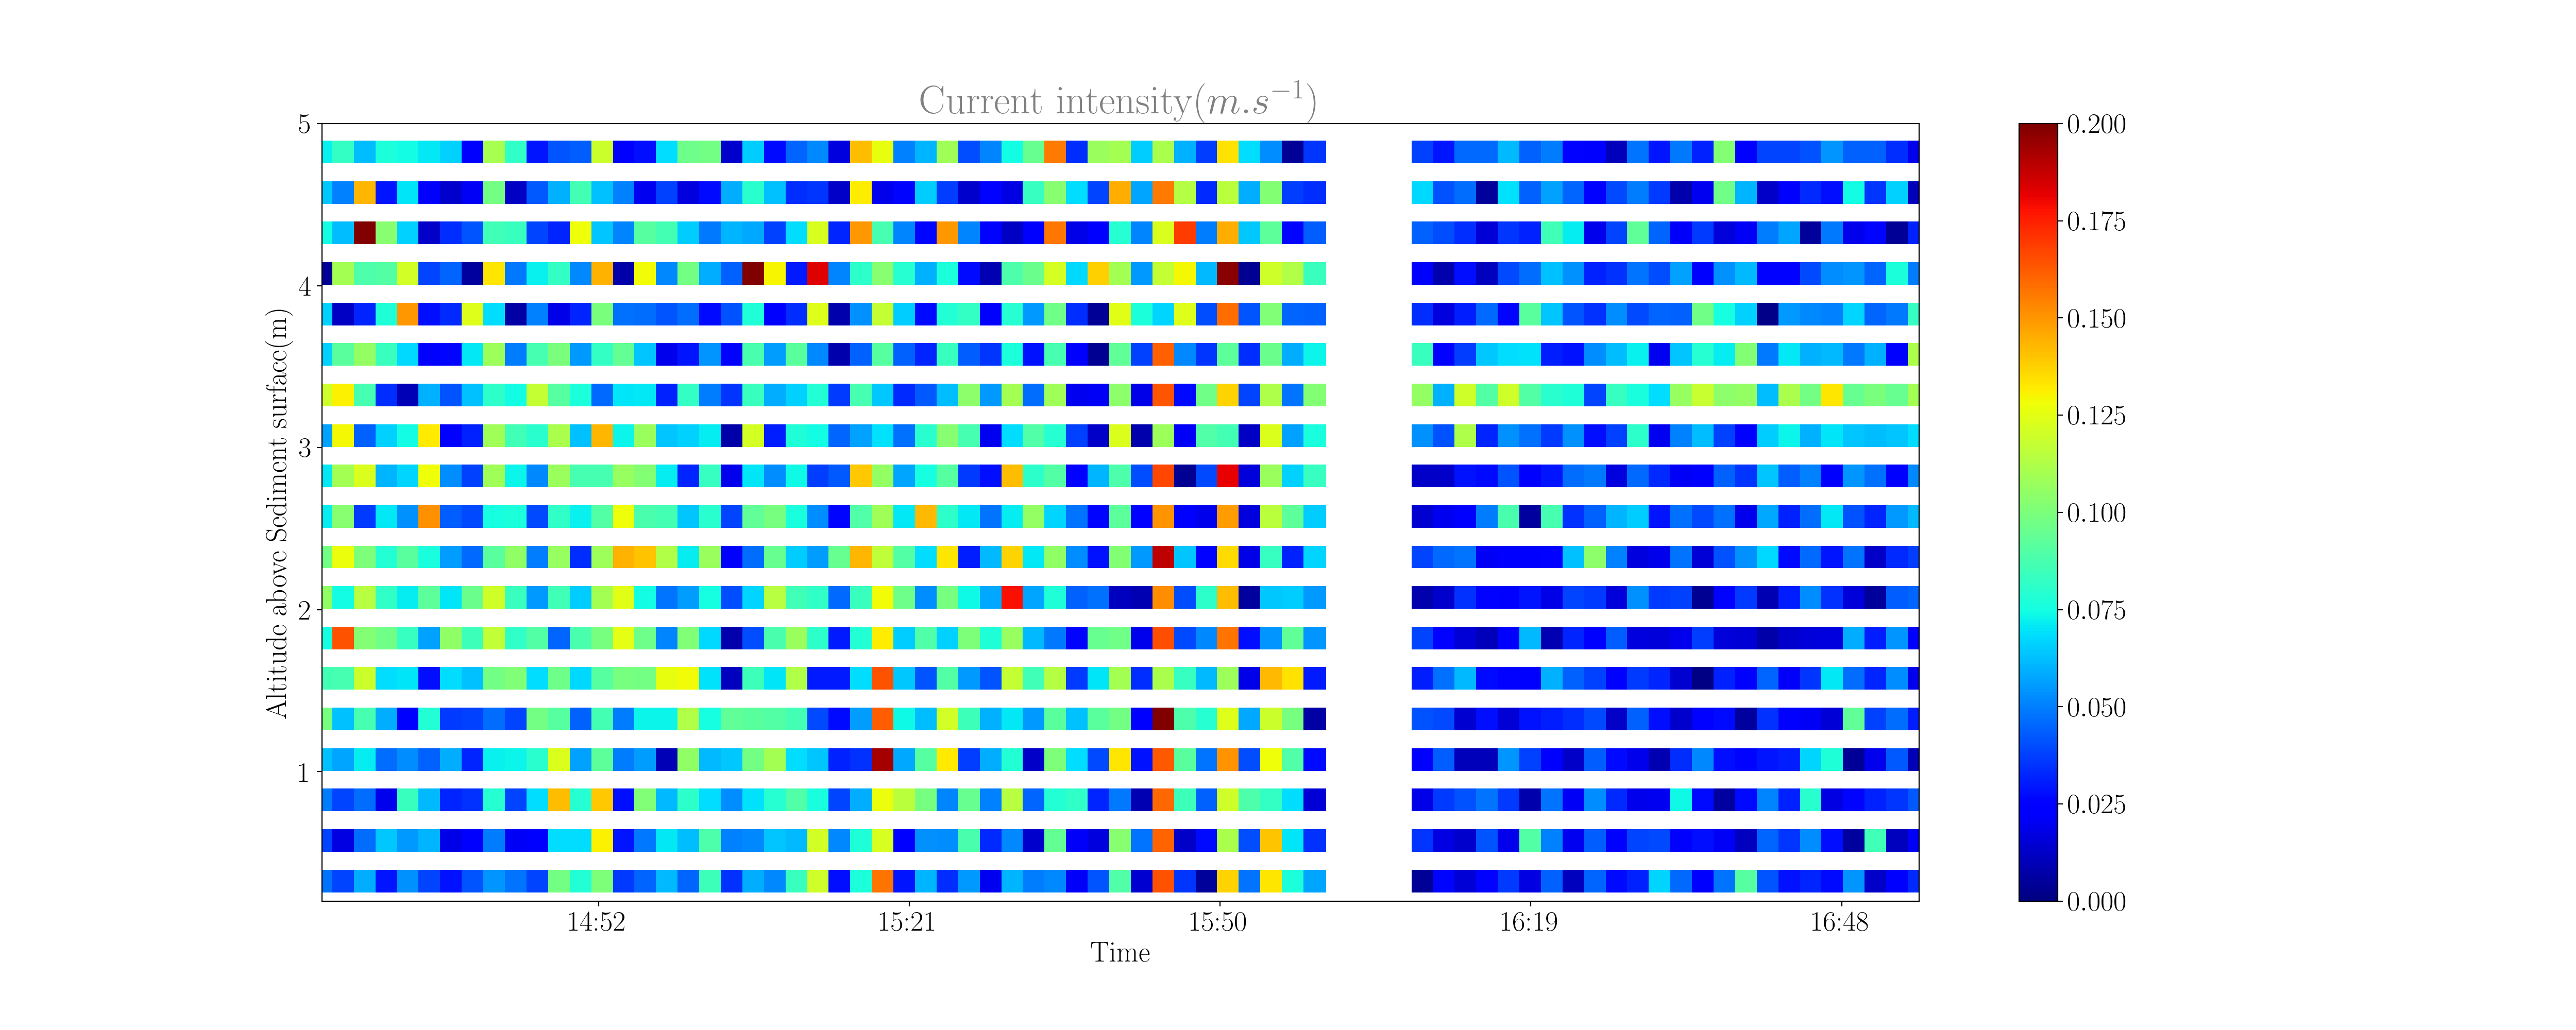
\includegraphics[width=0.8\textwidth]{1703F03scatterintensity.png}
		\caption{Intensité du courant de 14h30 à 16h50 ($m.s^{-1}$).}
	\end{center}
\end{figure}
\textbf{COM FIGURE 4} Pour le premier emplacement, l'intensité du courant peut plus ou moins être séparée en deux parties : pour les 20 premières minutes, les valeurs sont comprises entre 0,05 et 0,125 $m.s^{-1}$. Dans un second temps, l'intensité du courant augmente jusqu'à 0,175 $m.s^{-1}$, ce qui correspond au moment où le courant tourne en direction du Nord (figure 3).\\
\indent Pour le second emplacement, la direction du courant à la surface (entre 3 et 4 $m$ sur la figure 3) se situe entre 300°N et 350°N. En profondeur, le courant reste relativement orienté Nord avec des valeurs comprises entre 150°N et 350°N. \textbf{FIN COM FIGURE 4}\\

\begin{figure}[!ht]
	\begin{center}
		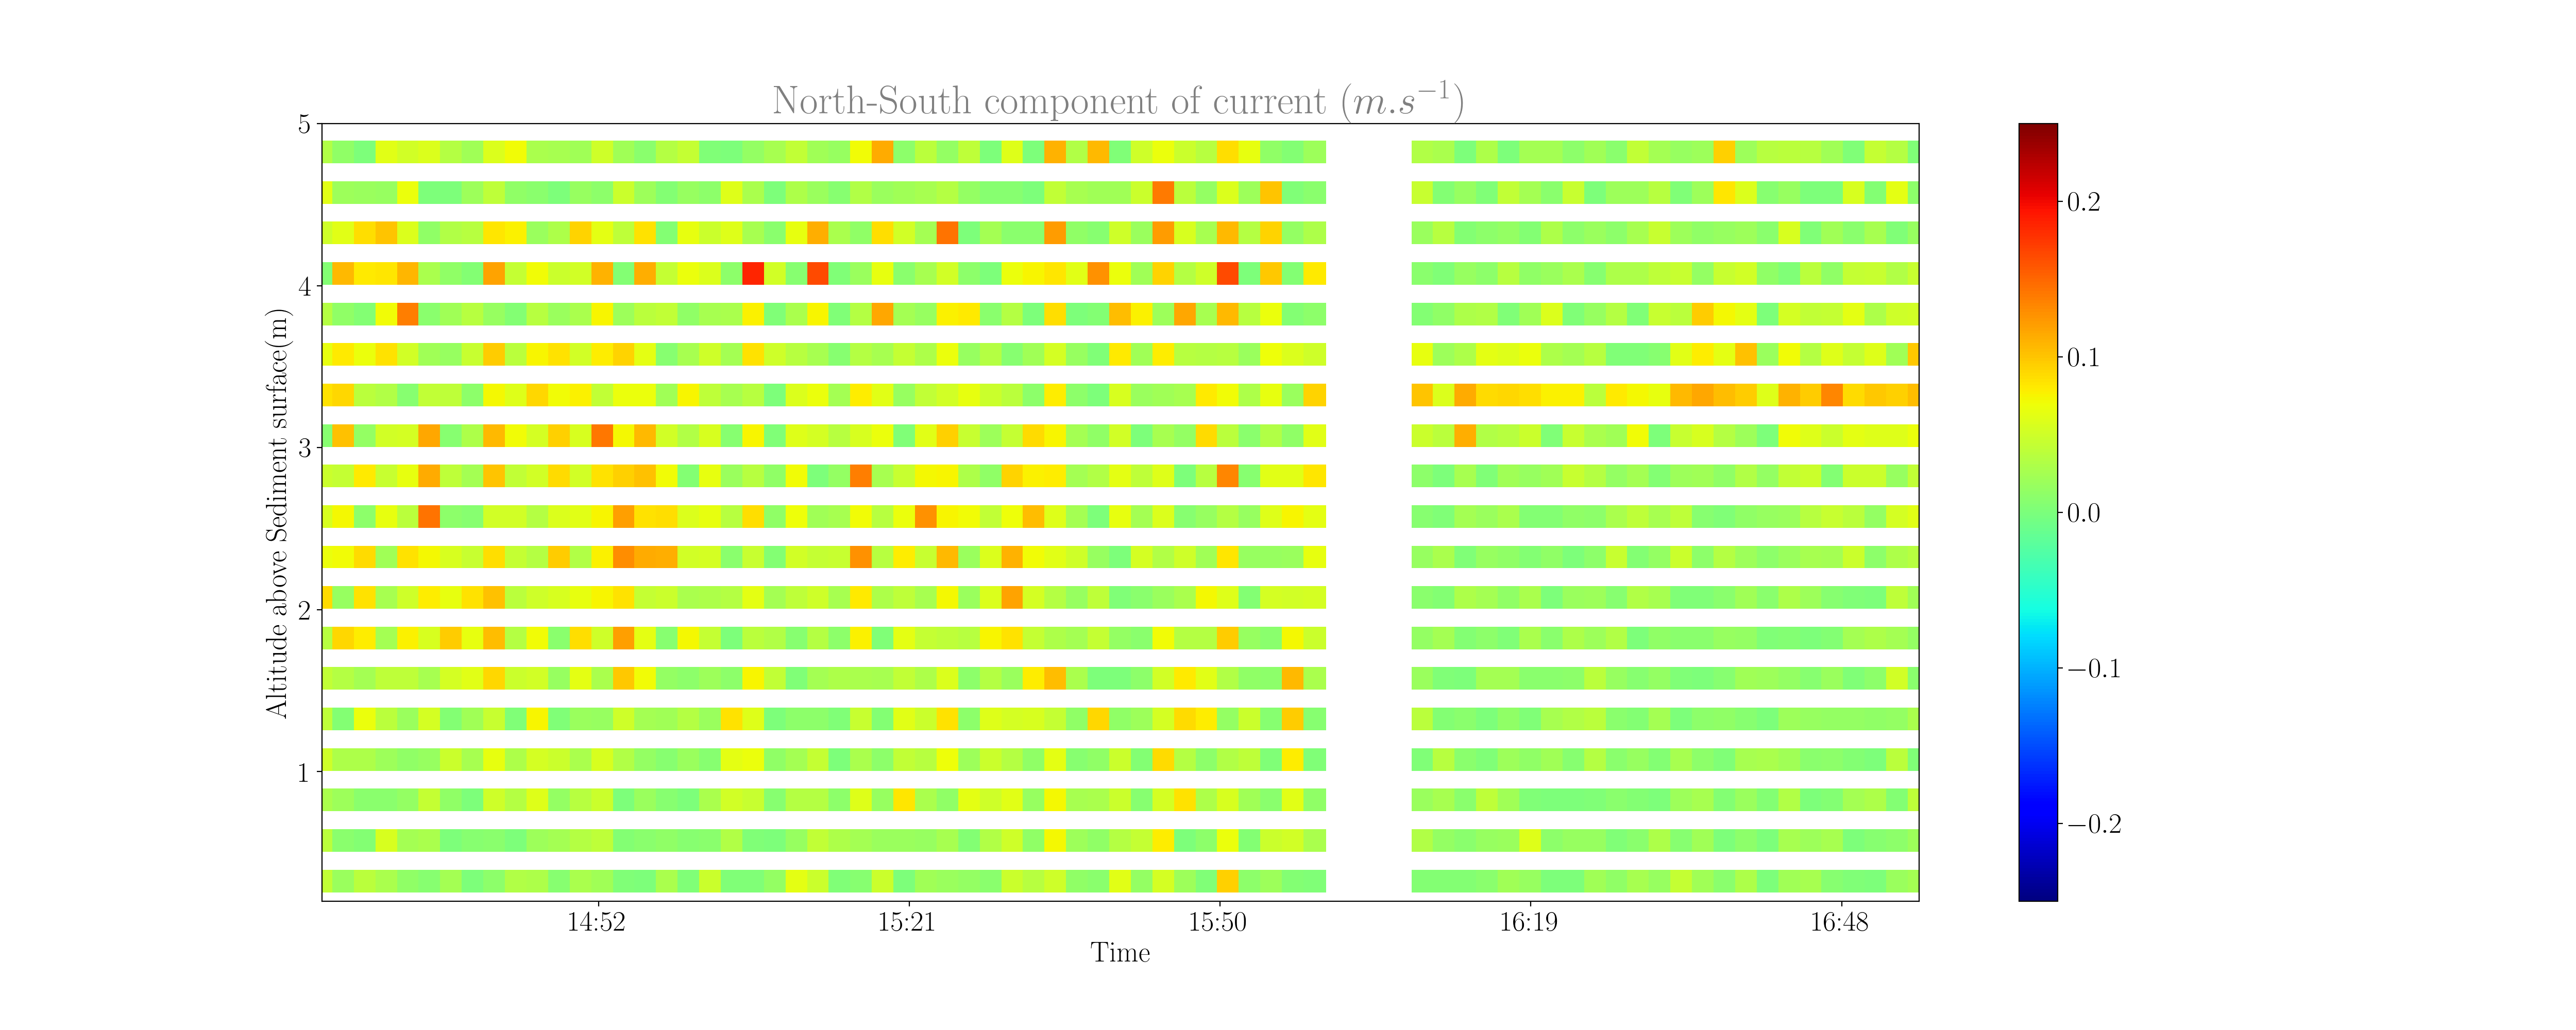
\includegraphics[width=0.8\textwidth]{1703F03scatterv2.png}
		\caption{Intensité du courant selon la composante Nord-Sud de 14h30 à 16h50 ($m.s^{-1}$).}
	\end{center}
\end{figure}
\textbf{COM FIGURE 5} Pour le premier emplacement, la vitesse du courant selon la composante Nord-Sud semble augmenter à la surface.\\
\indent Pour le second emplacement, la vitesse du courant à la surface (entre 3 et 4 $m$ sur la figure 3) se situe autour de 0,1 $m.s^{-1}$. En profondeur, la vitesse reste quasiment nulle. \textbf{FIN COM FIGURE 5}\\

\begin{figure}[!ht]
	\begin{center}
		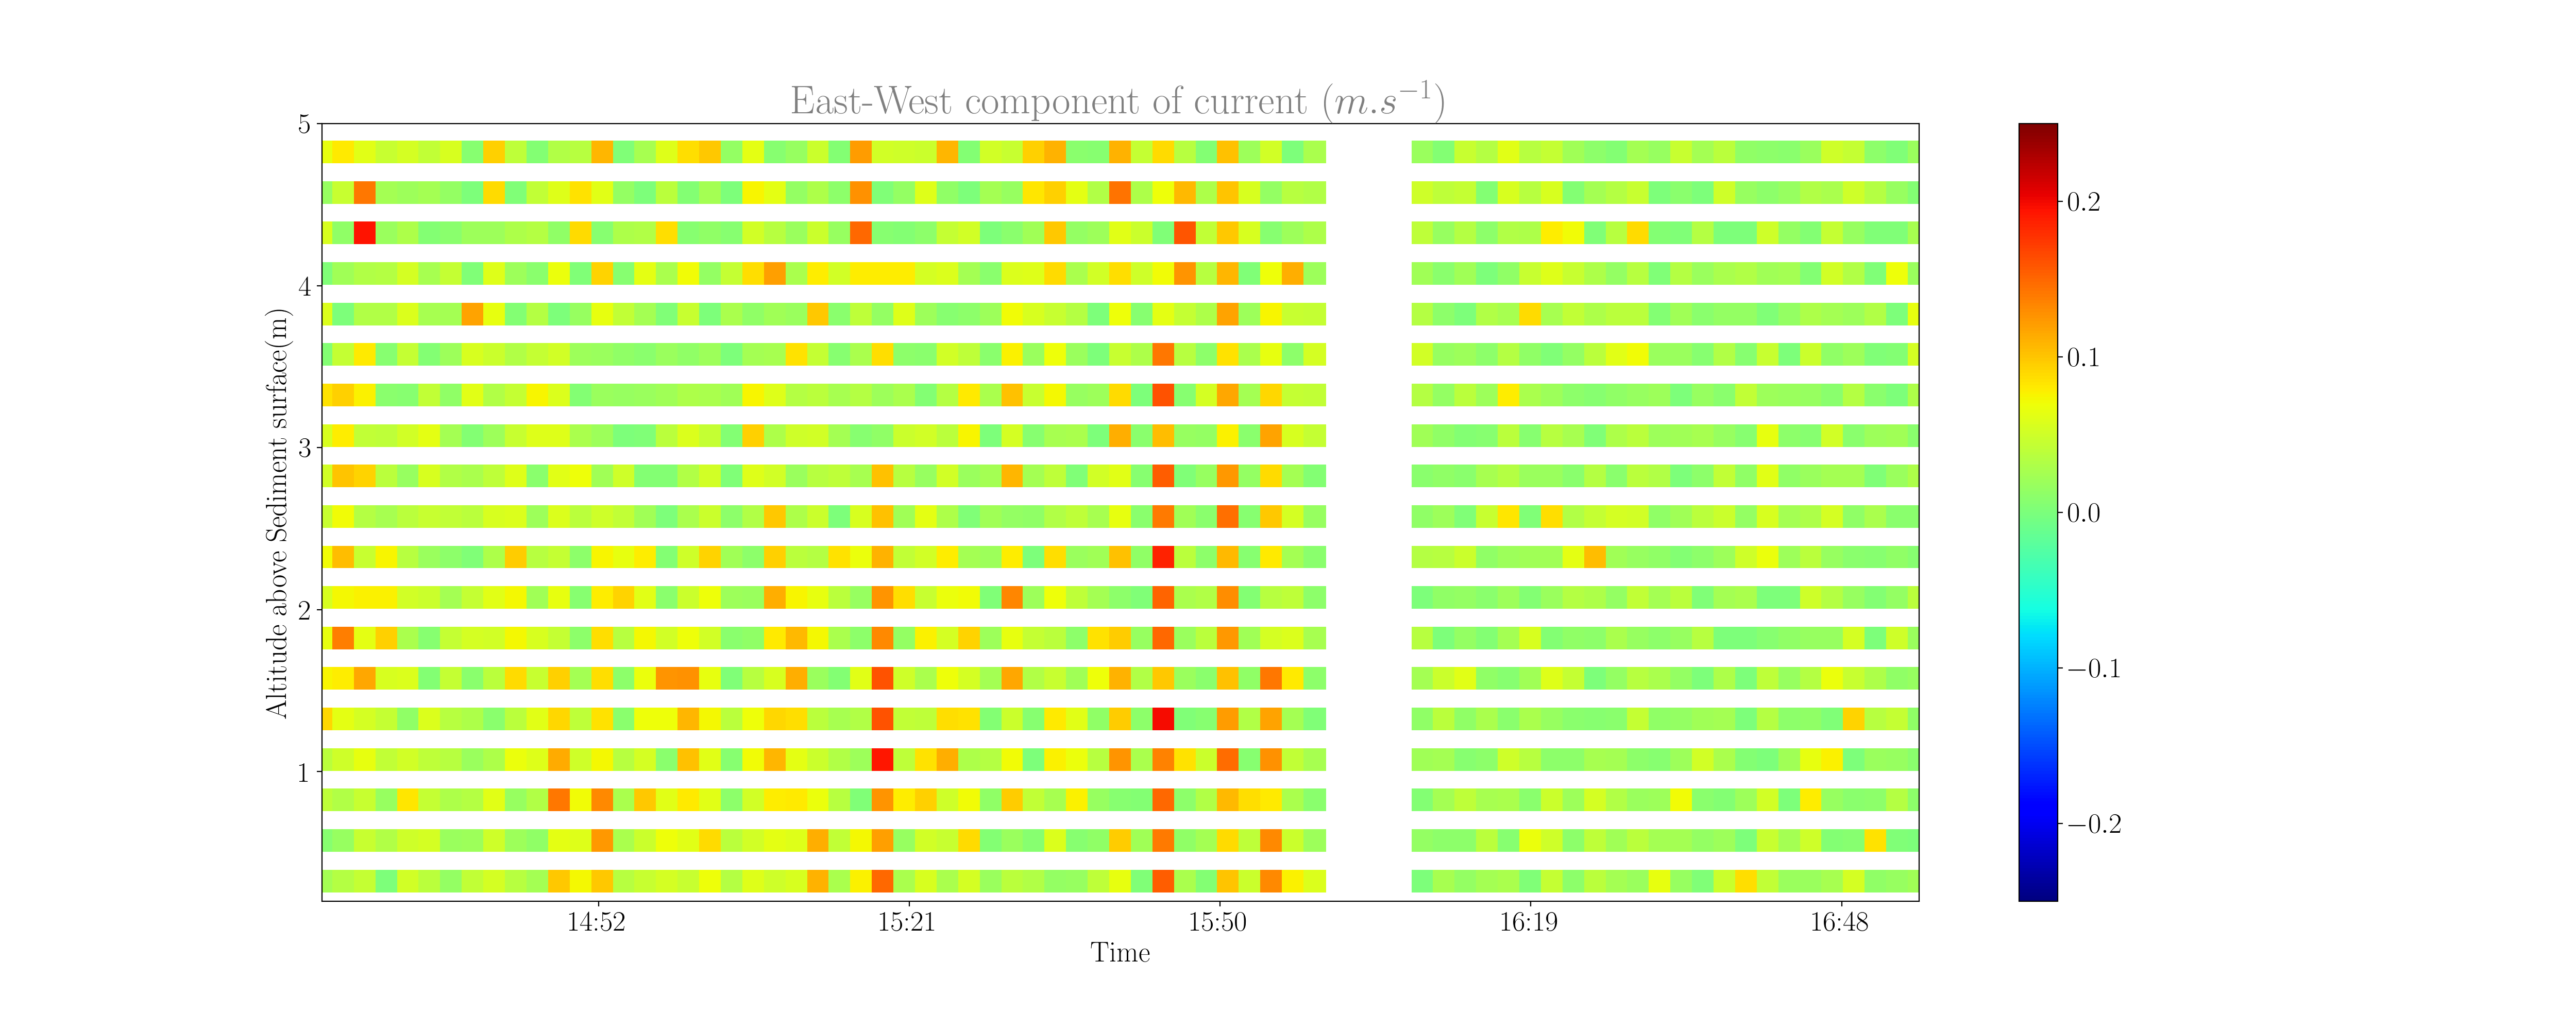
\includegraphics[width=0.8\textwidth]{1703F03scatterv1.png}
		\caption{Intensité du courant selon la composante Est-Ouest de 14h30 à 16h50 ($m.s^{-1}$).}
	\end{center}
\end{figure}
\textbf{COM FIGURE 6} Pour le premier emplacement, la vitesse du courant selon la composante Est-Ouest semble augmenter dans la colonne dans un second temps.\\
\indent Pour le second emplacement, la vitesse du courant reste majoritairement nulle avec quelques points allant jusqu'à 0,1 $m.s^{-1}$. \textbf{FIN COM FIGURE 6}\\
\clearpage 

\subsection{Journée du 18 mars 2021}
\subsubsection{Emplacement 1}

\begin{figure}[!ht]
	\begin{center}
	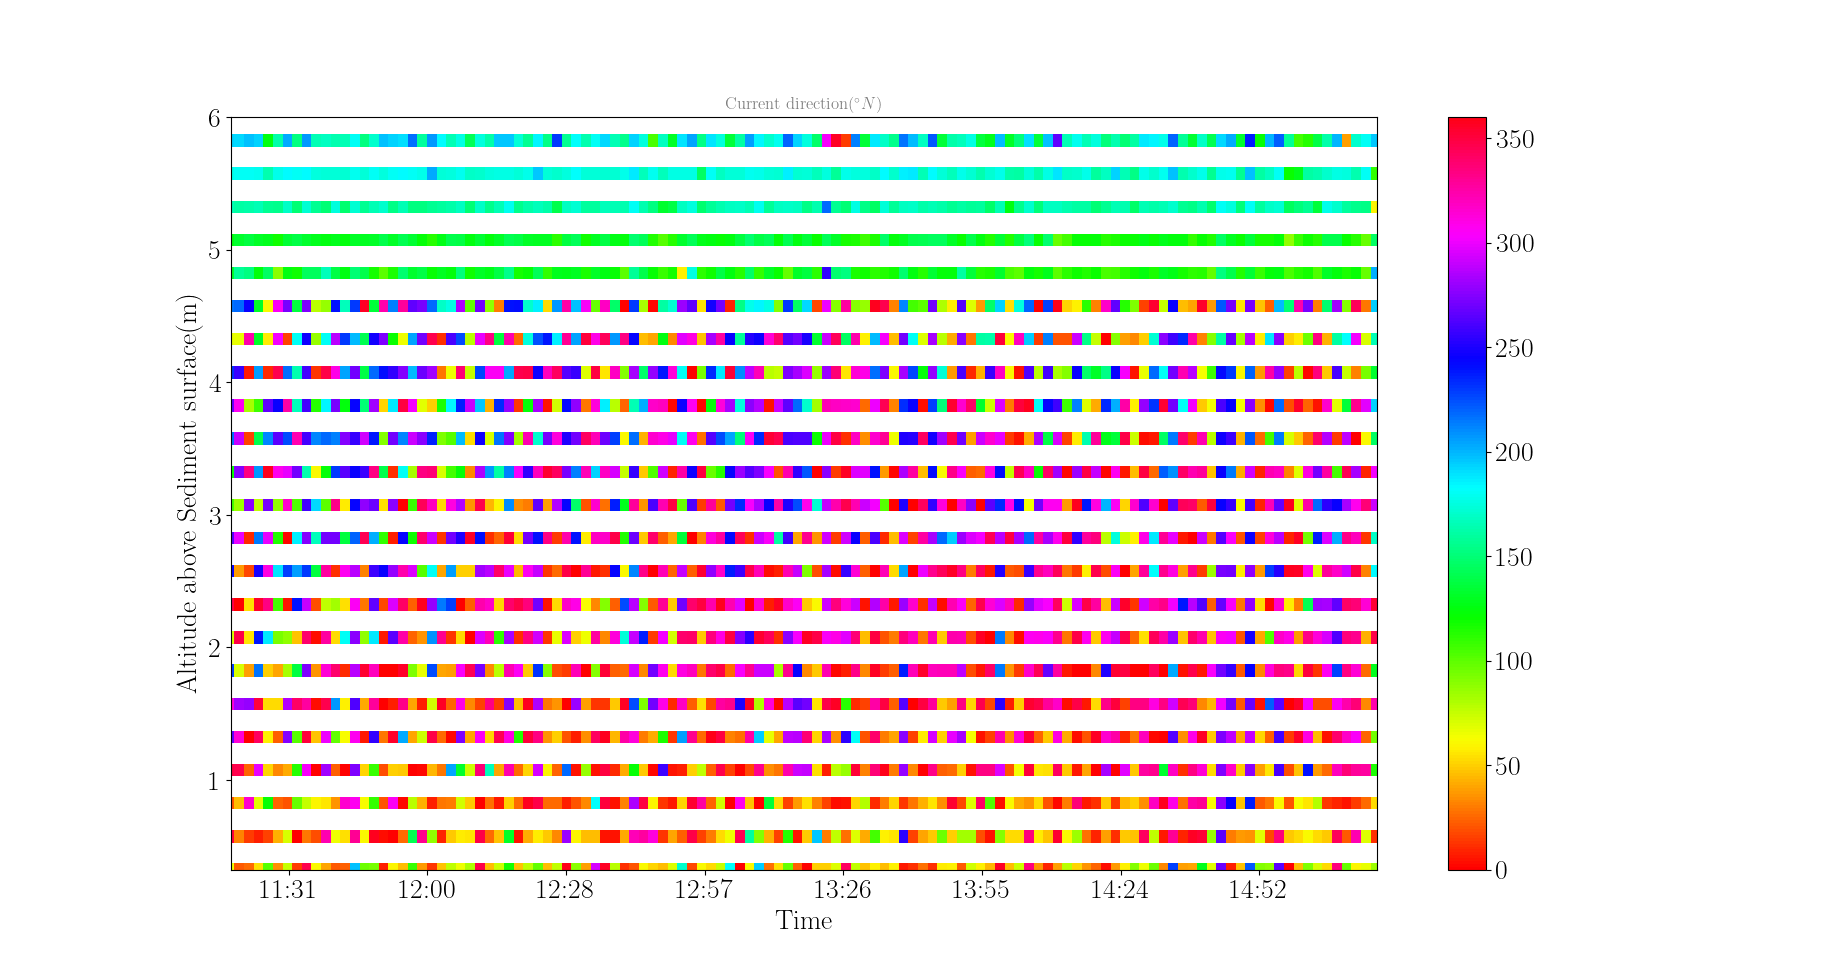
\includegraphics[width=0.8\textwidth]{180321021scatterdirection.png}
	\caption{Direction du courant de 11h18 à 15h19 ($^{\circ}$N).}
	\end{center}
\end{figure}
La colonne d'eau peut être divisée en deux parties : de la surface à un mètre de profondeur (entre 5 et 6 $m$ au-dessus du fond) la direction varie entre 125 $^{\circ}$N et 175 $^{\circ}$N tout en étant stable au cours du temps.
De 4,7 $m$ au-dessus du fond et jusqu'au fond, le courant varie entre 300 $^{\circ}$N et 360 $^{\circ}$N avec un profil temporel stable.\\

\begin{figure}[!ht]
	\begin{center}
		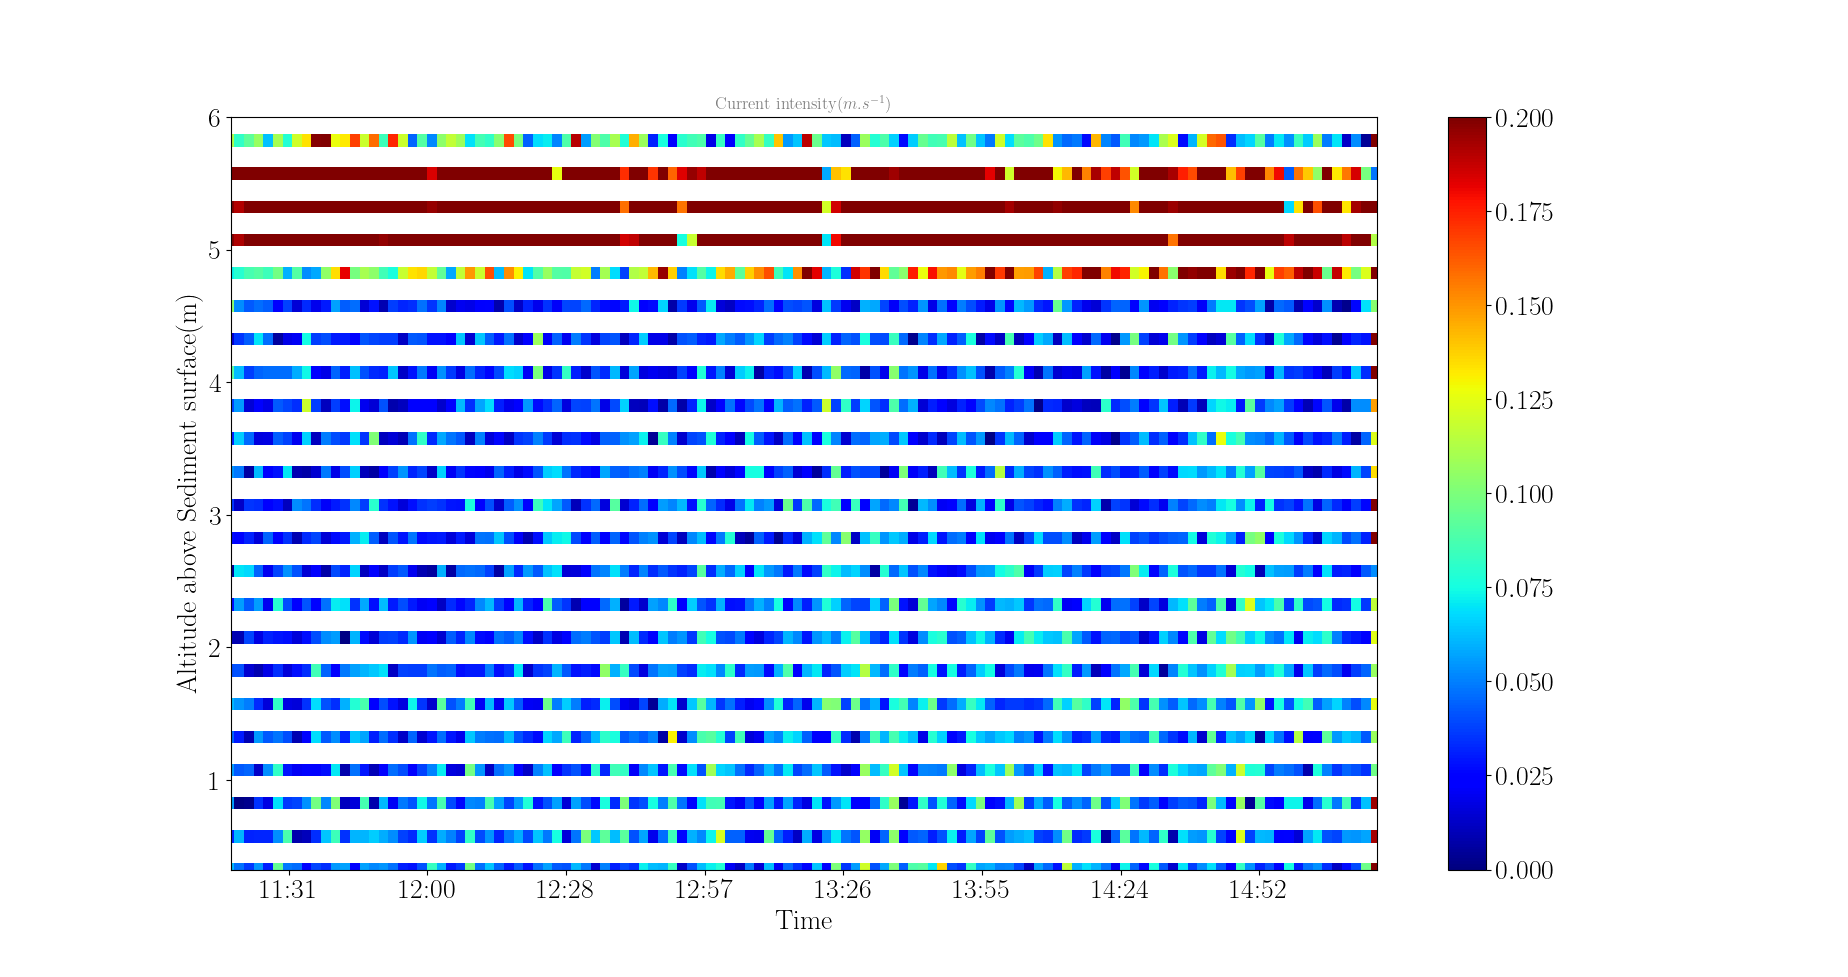
\includegraphics[width=0.8\textwidth]{180321021scatterintensity.png}
		\caption{Intensité du courant de 11h18 à 15h19 ($m.s^{-1}$).}
	\end{center}
\end{figure}
La colonne d'eau peut être divisée en deux zones selon son intensité. Entre la surface et un mètre de profondeur l'intensité du courant ne présente que peu de variation temporelle avec des valeurs se situant entre 0,175 $m.s^{-1}$ et 0,2 $m.s^{-1}$. De 4,7 $m$ au-dessus du fond et jusqu'au fond, l'intensité est faible et présente peu de variation temporelle avec des valeurs comprises entre 0,025 $m.s^{-1}$ et 0,075 $m.s^{-1}$.\\

\begin{figure}[!ht]
	\begin{center}
		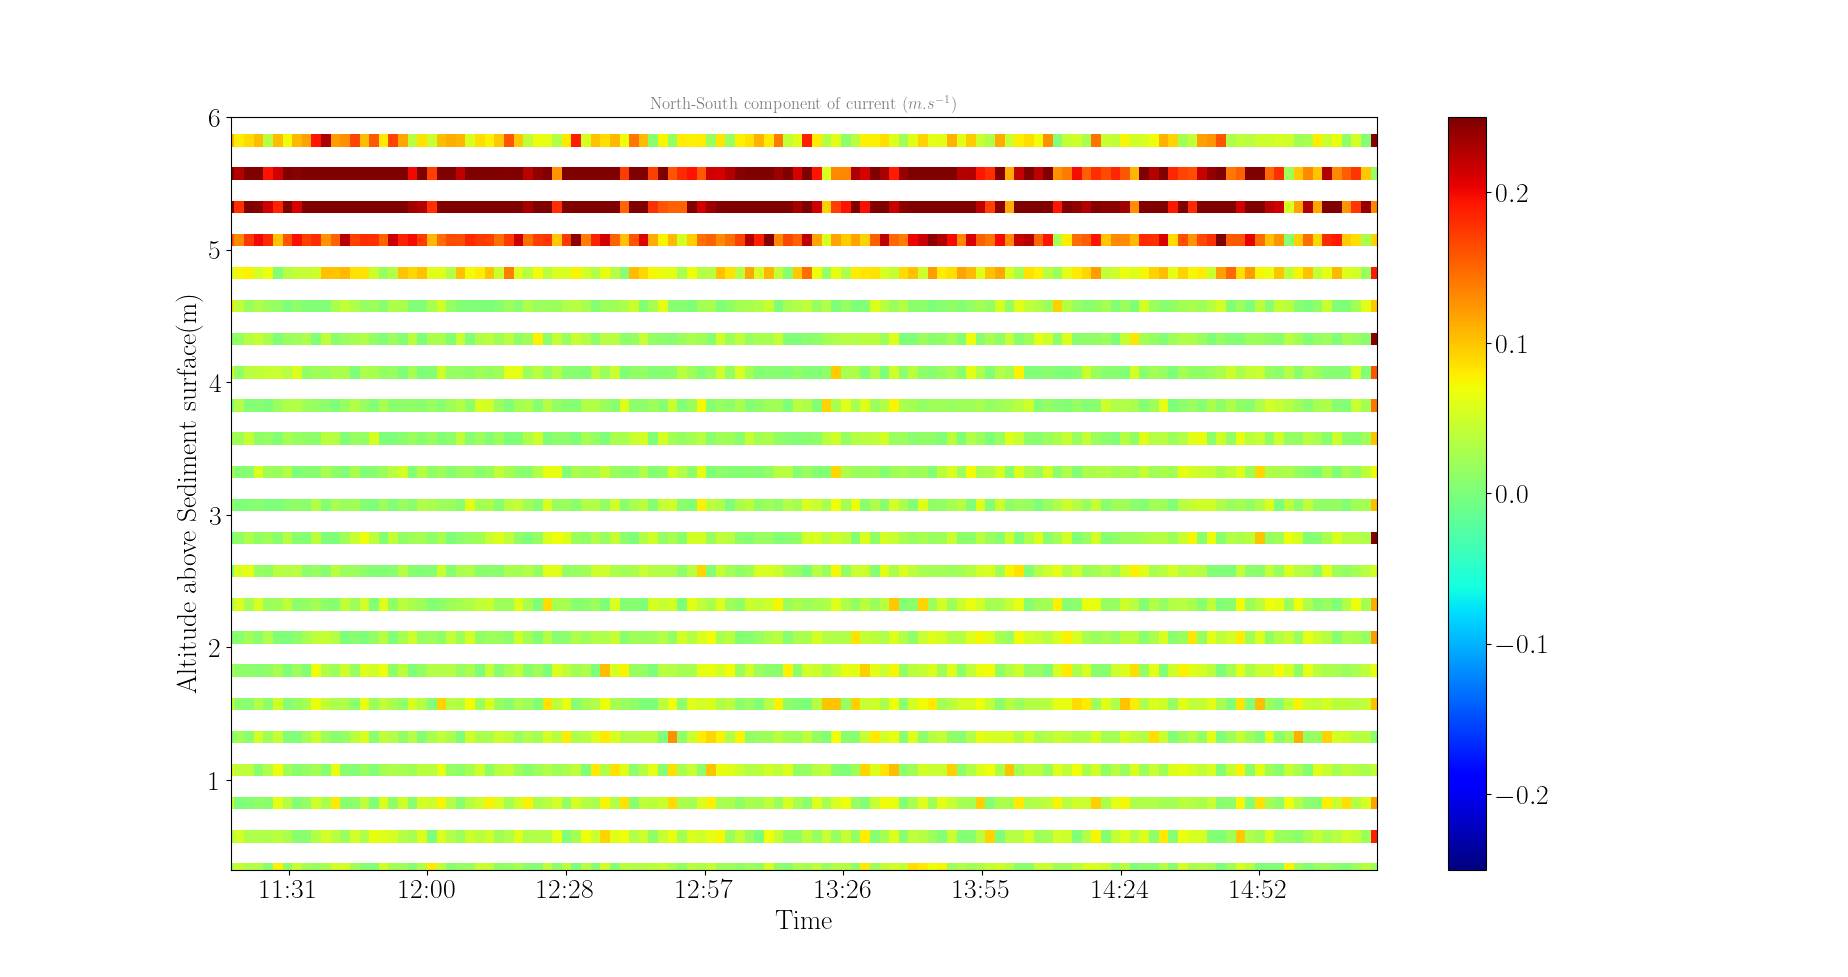
\includegraphics[width=0.8\textwidth]{180321021scatterv2.png}
		\caption{Intensité du courant selon la composante Nord-Sud de 11h18 à 15h19 ($m.s^{-1}$).}
	\end{center}
\end{figure}
L'intensité du courant selon la composante Nord-Sud ne présente sur la période temporelle qu'une seule strate notoire, entre 5 $m$ et 6 $m$ au-dessus du fond (à la surface et subsurface), avec des intensités comprises entre 0,15 $m.s^{-1}$ et 0,25 $m.s^{-1}$.\\

\begin{figure}[!ht]
	\begin{center}
		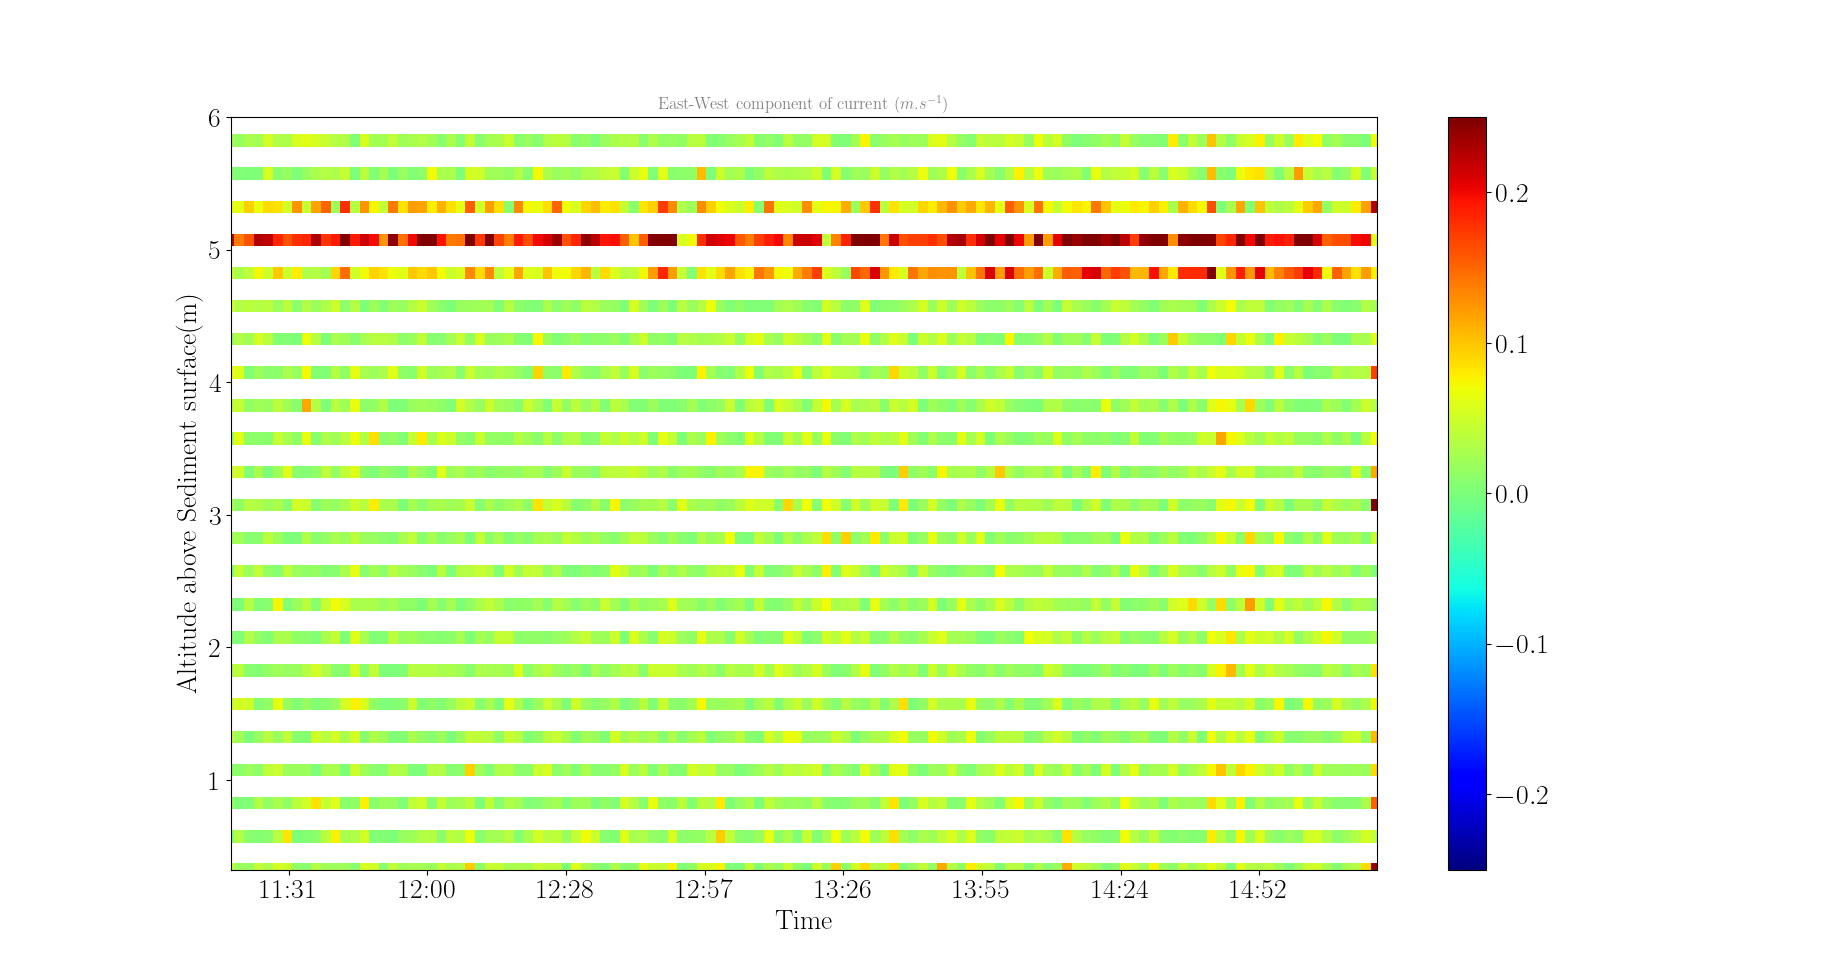
\includegraphics[width=0.8\textwidth]{180321021scatterv1.png}
		\caption{Intensité du courant selon la composante Est-Ouest de 11h18 à 15h19 ($m.s^{-1}$).}
	\end{center}
\end{figure}
L'intensité du courant selon la composante Est-Ouest ne présente sur la période temporelle qu'une seule strate notoire, entre 4,9 $m$ et 5 $m$ au-dessus du fond (subsurface), avec des intensités comprises entre 0,15 $m.s^{-1}$ et 0,25 $m.s^{-1}$.\\

\begin{figure}[!ht]
	\begin{center}
		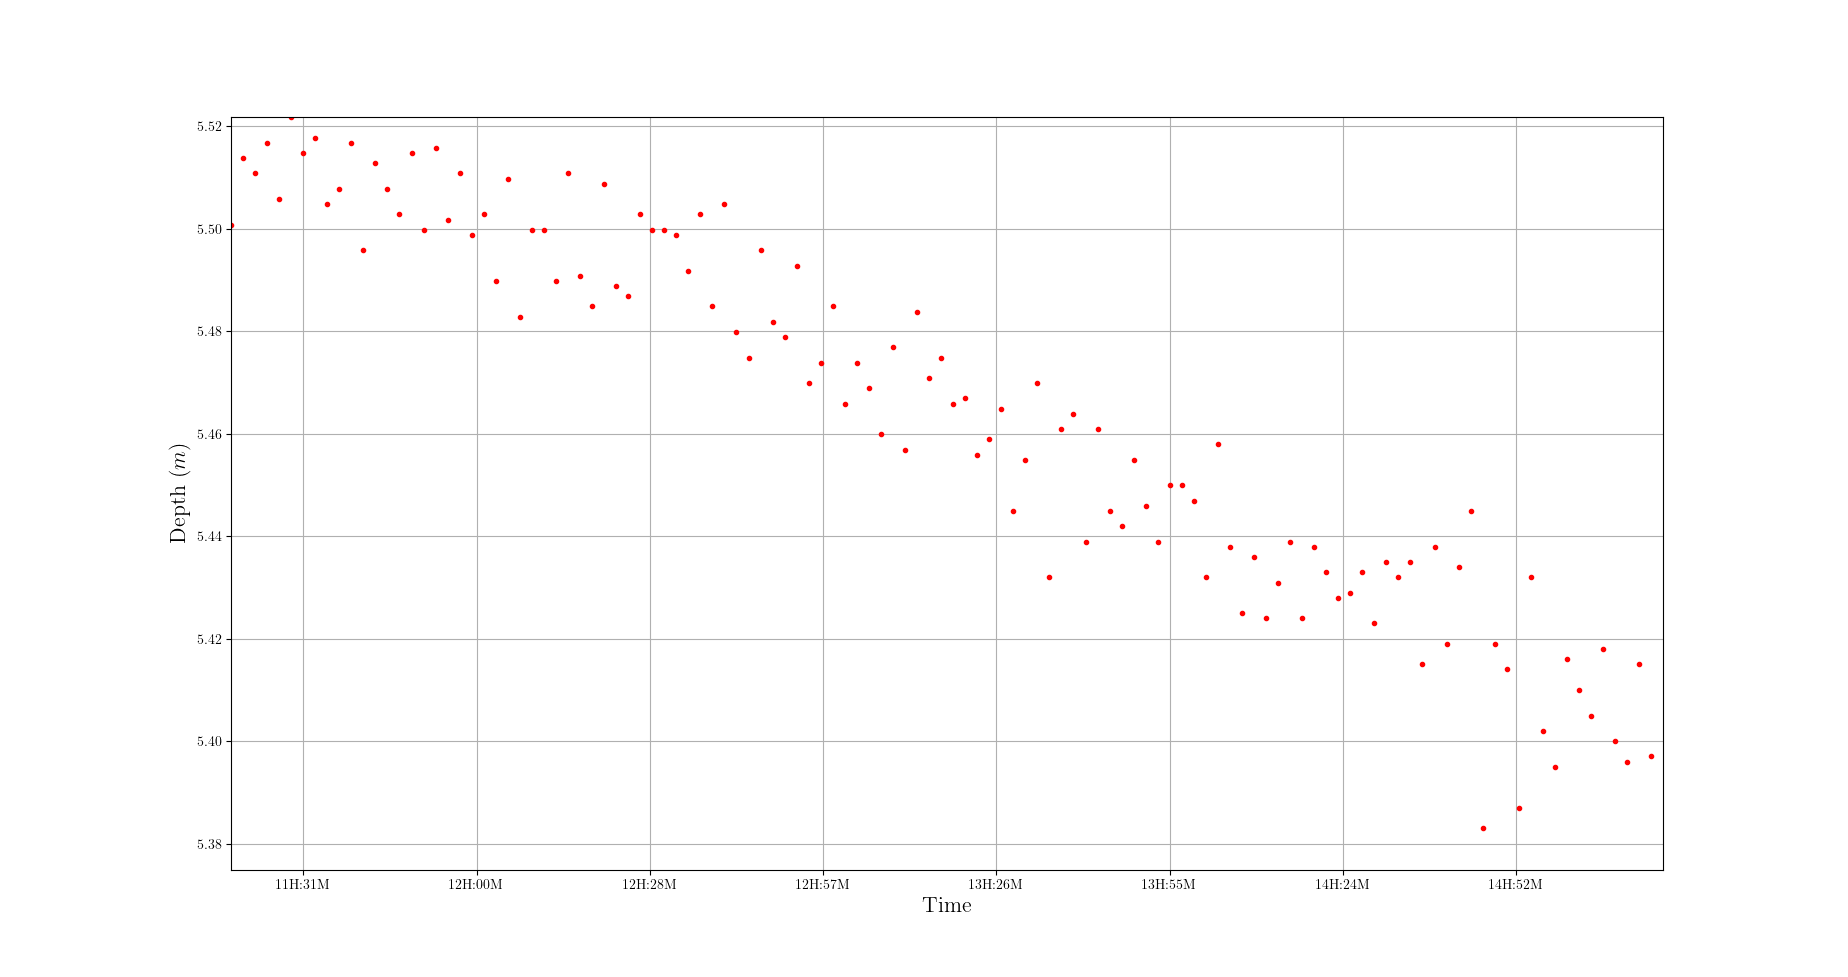
\includegraphics[width=0.8\textwidth]{Figure_2.png}
		\caption{Profondeur mesurée d'immersion de l'Aquadopp ($m$).}
	\end{center}
\end{figure}
La profondeur d'immersion mesurée par l'Aquadopp a baissé au cours du temps malgré une position immobile. En effet, les valeurs de profondeur varient de 5,52 $m$ à 5,38 $m$ au-dessus du fond. Cela est dû au phénomène de marée léger mais présent en Méditerranée.

\subsubsection{Emplacement 2}
L'Aquadopp a été immergé ici afin de voir l'effet potentiel des cages de la ferme aquacole du Frioul (+ blabla) sur le courant en comparaison avec le premier emplacement. Mais le temps d'immersion de 50 minutes.\\

\begin{figure}[!ht]
	\begin{center}
		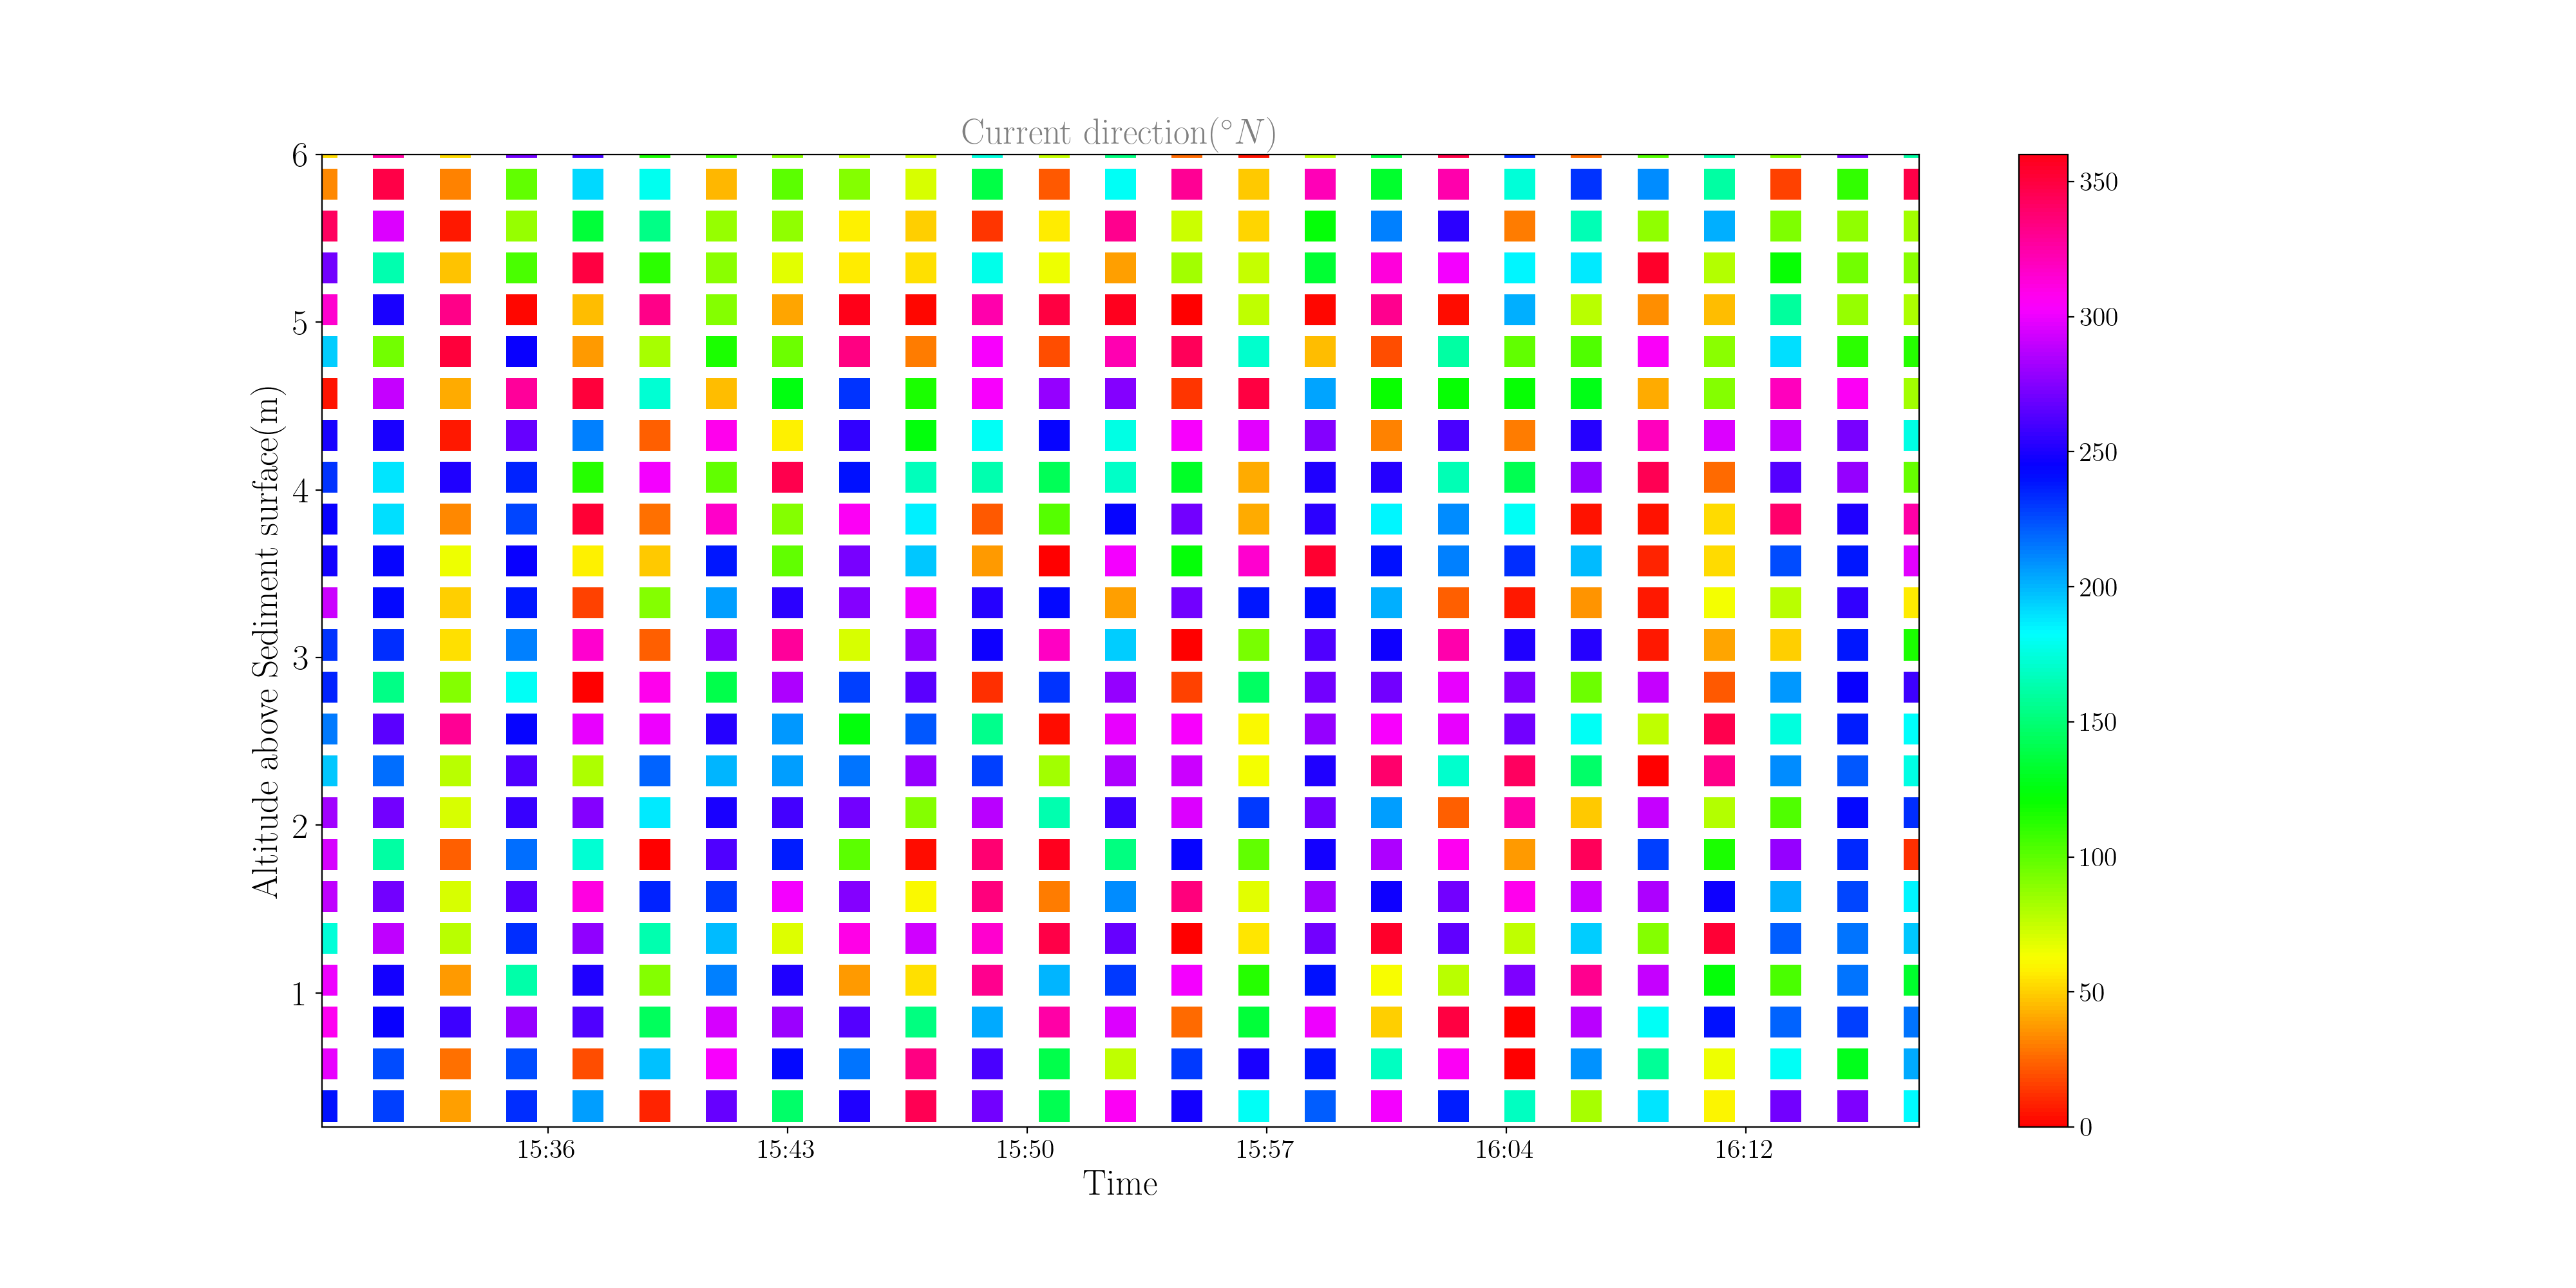
\includegraphics[width=0.8\textwidth]{18032102scatterdirection.png}
		\caption{Direction du courant de 15h30 à 16h20 ($^{\circ}$N).}
	\end{center}
\end{figure}
Une bière à celui qui commente cette figure

\begin{figure}[!ht]
	\begin{center}
		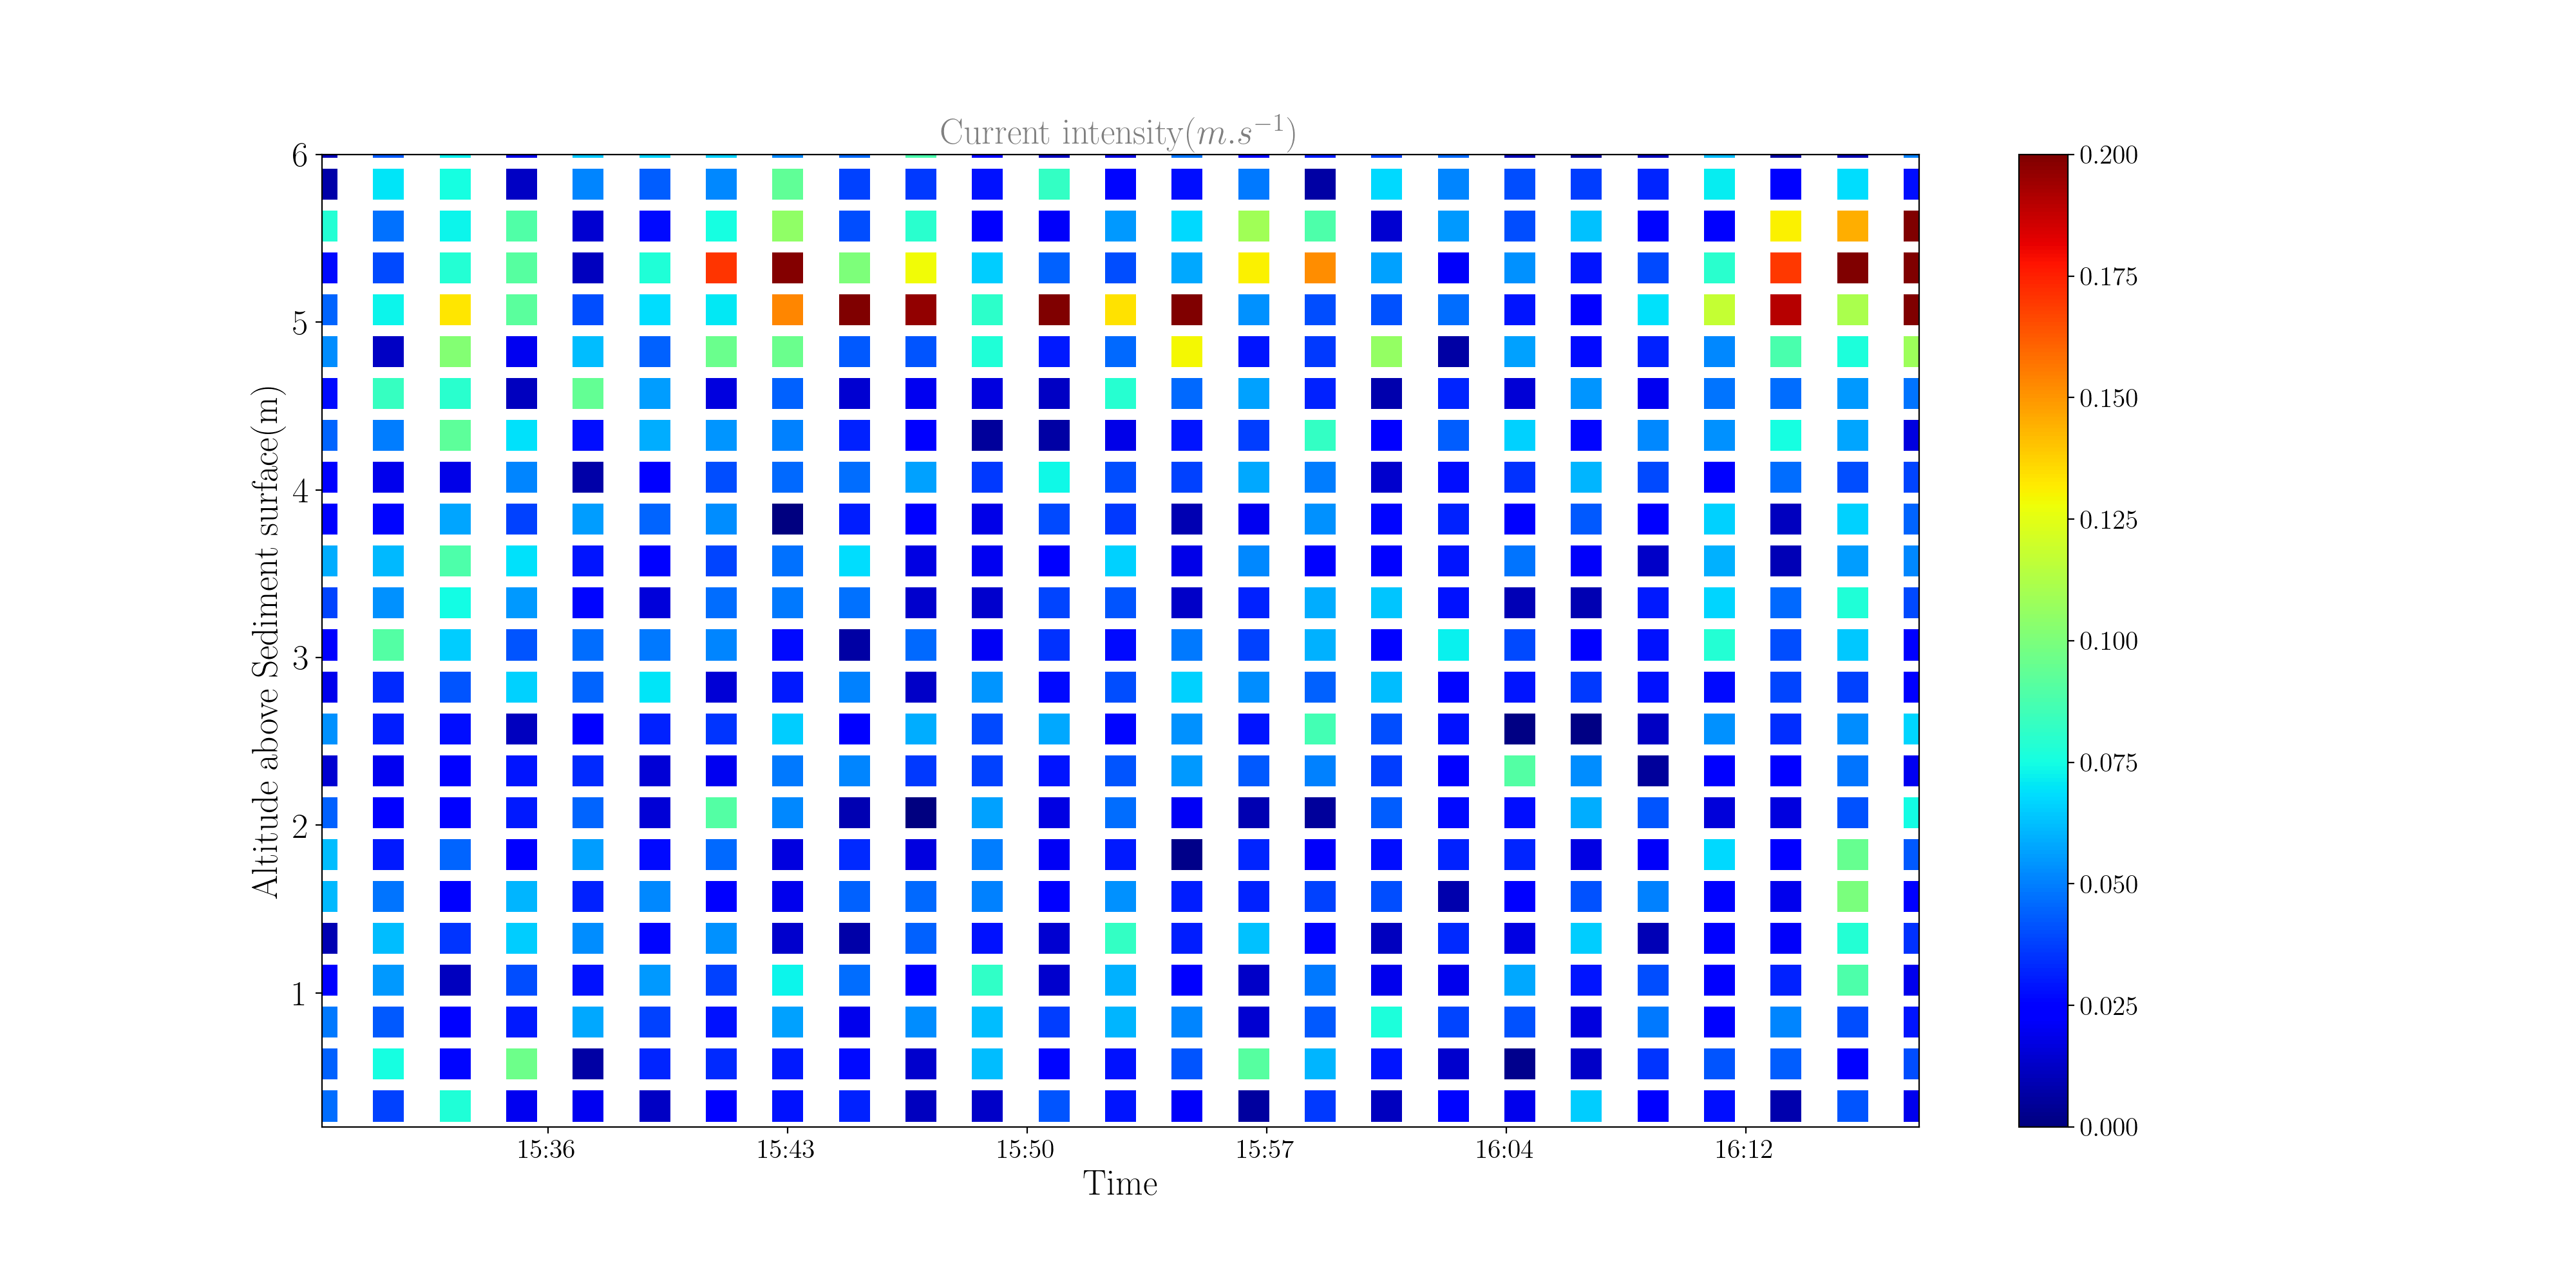
\includegraphics[width=0.8\textwidth]{18032102scatterintensity.png}
		\caption{Intensité du courant de 15h30 à 16h20 ($m.s^{-1}$).}
	\end{center}
\end{figure}
Ici (figure 8), le profil est moins net à cause du temps réduit d'immersion de l'Aquadopp. Néanmoins, la colonne d'eau peut être divisée en deux zones selon son intensité. A la surface, autour de 5 $m$ et jusqu'à 6 $m$ au-dessus du fond, l'intensité du courant atteint son maximum avec des valeurs se situant entre 0,125 $m.s^{-1}$ et 0,2 $m.s^{-1}$. Puis l'intensité diminue jusqu'au fond avec des valeurs comprises entre 0 $m.s^{-1}$ et 0,075 $m.s^{-1}$ environ.\\

\begin{figure}[!ht]
	\begin{center}
		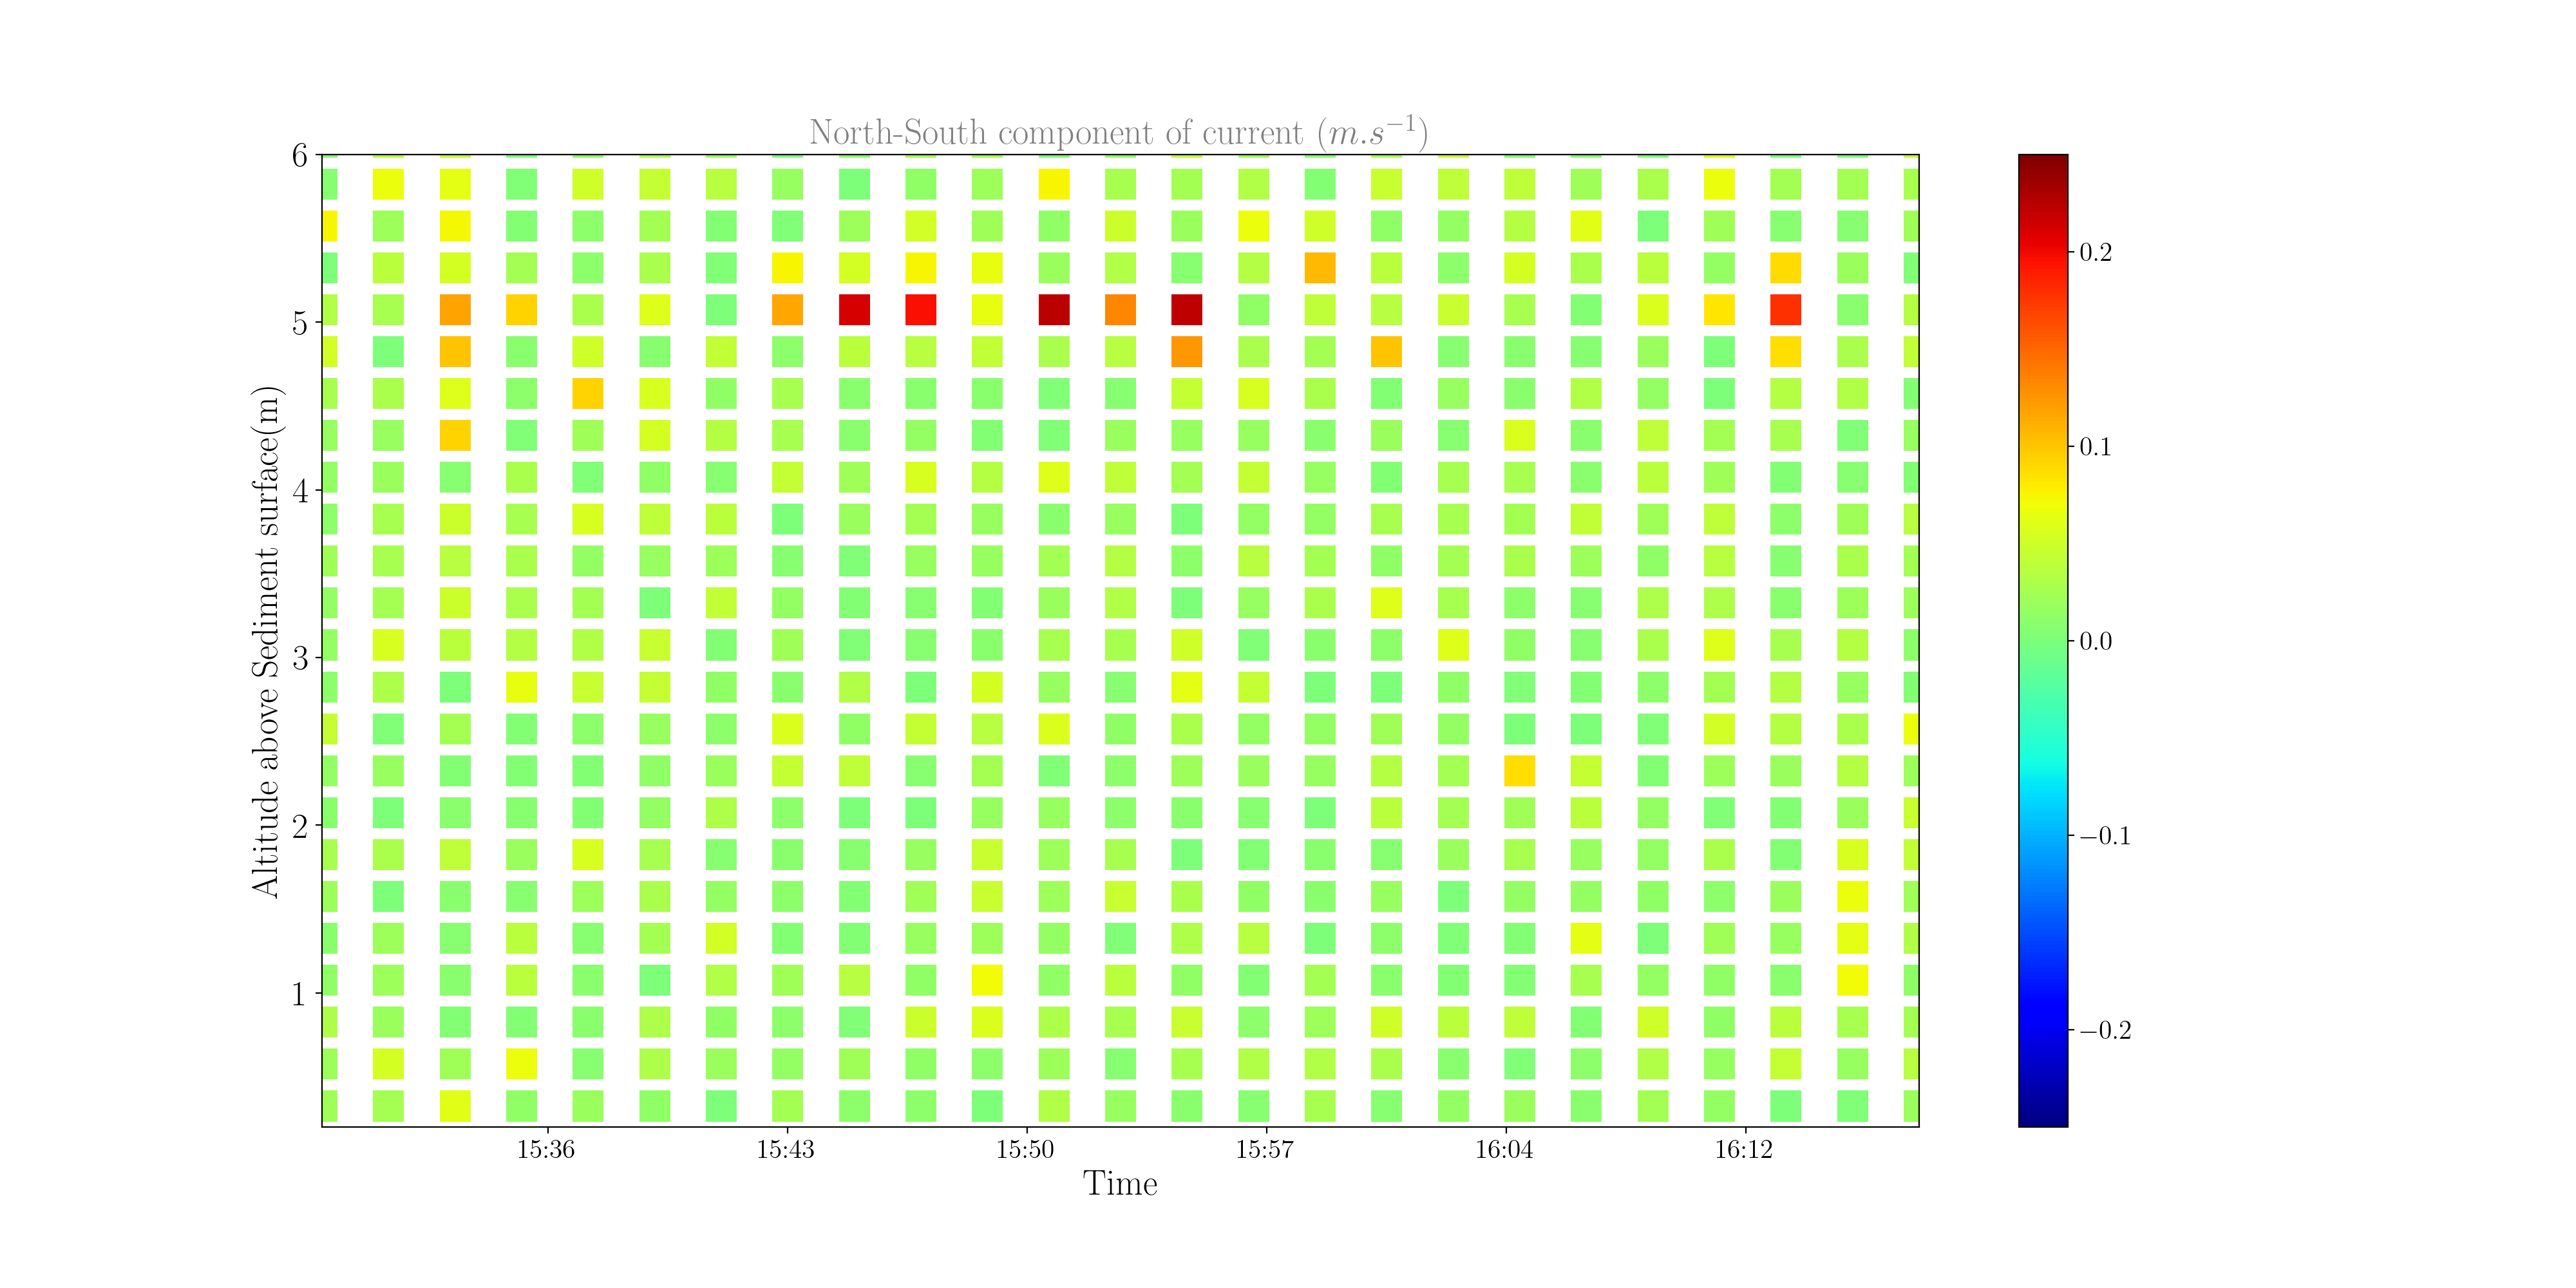
\includegraphics[width=0.8\textwidth]{18032102scatterv2.png}
		\caption{Intensité du courant selon la composante Nord-Sud de 15h30 à 16h20 ($m.s^{-1}$).}
	\end{center}
\end{figure}
L'intensité du courant selon la composante Nord-Sud est comprise entre 0,1 $m.s^{-1}$ et 0,25 $m.s^{-1}$ à la surface.\\

\begin{figure}[!ht]
	\begin{center}
		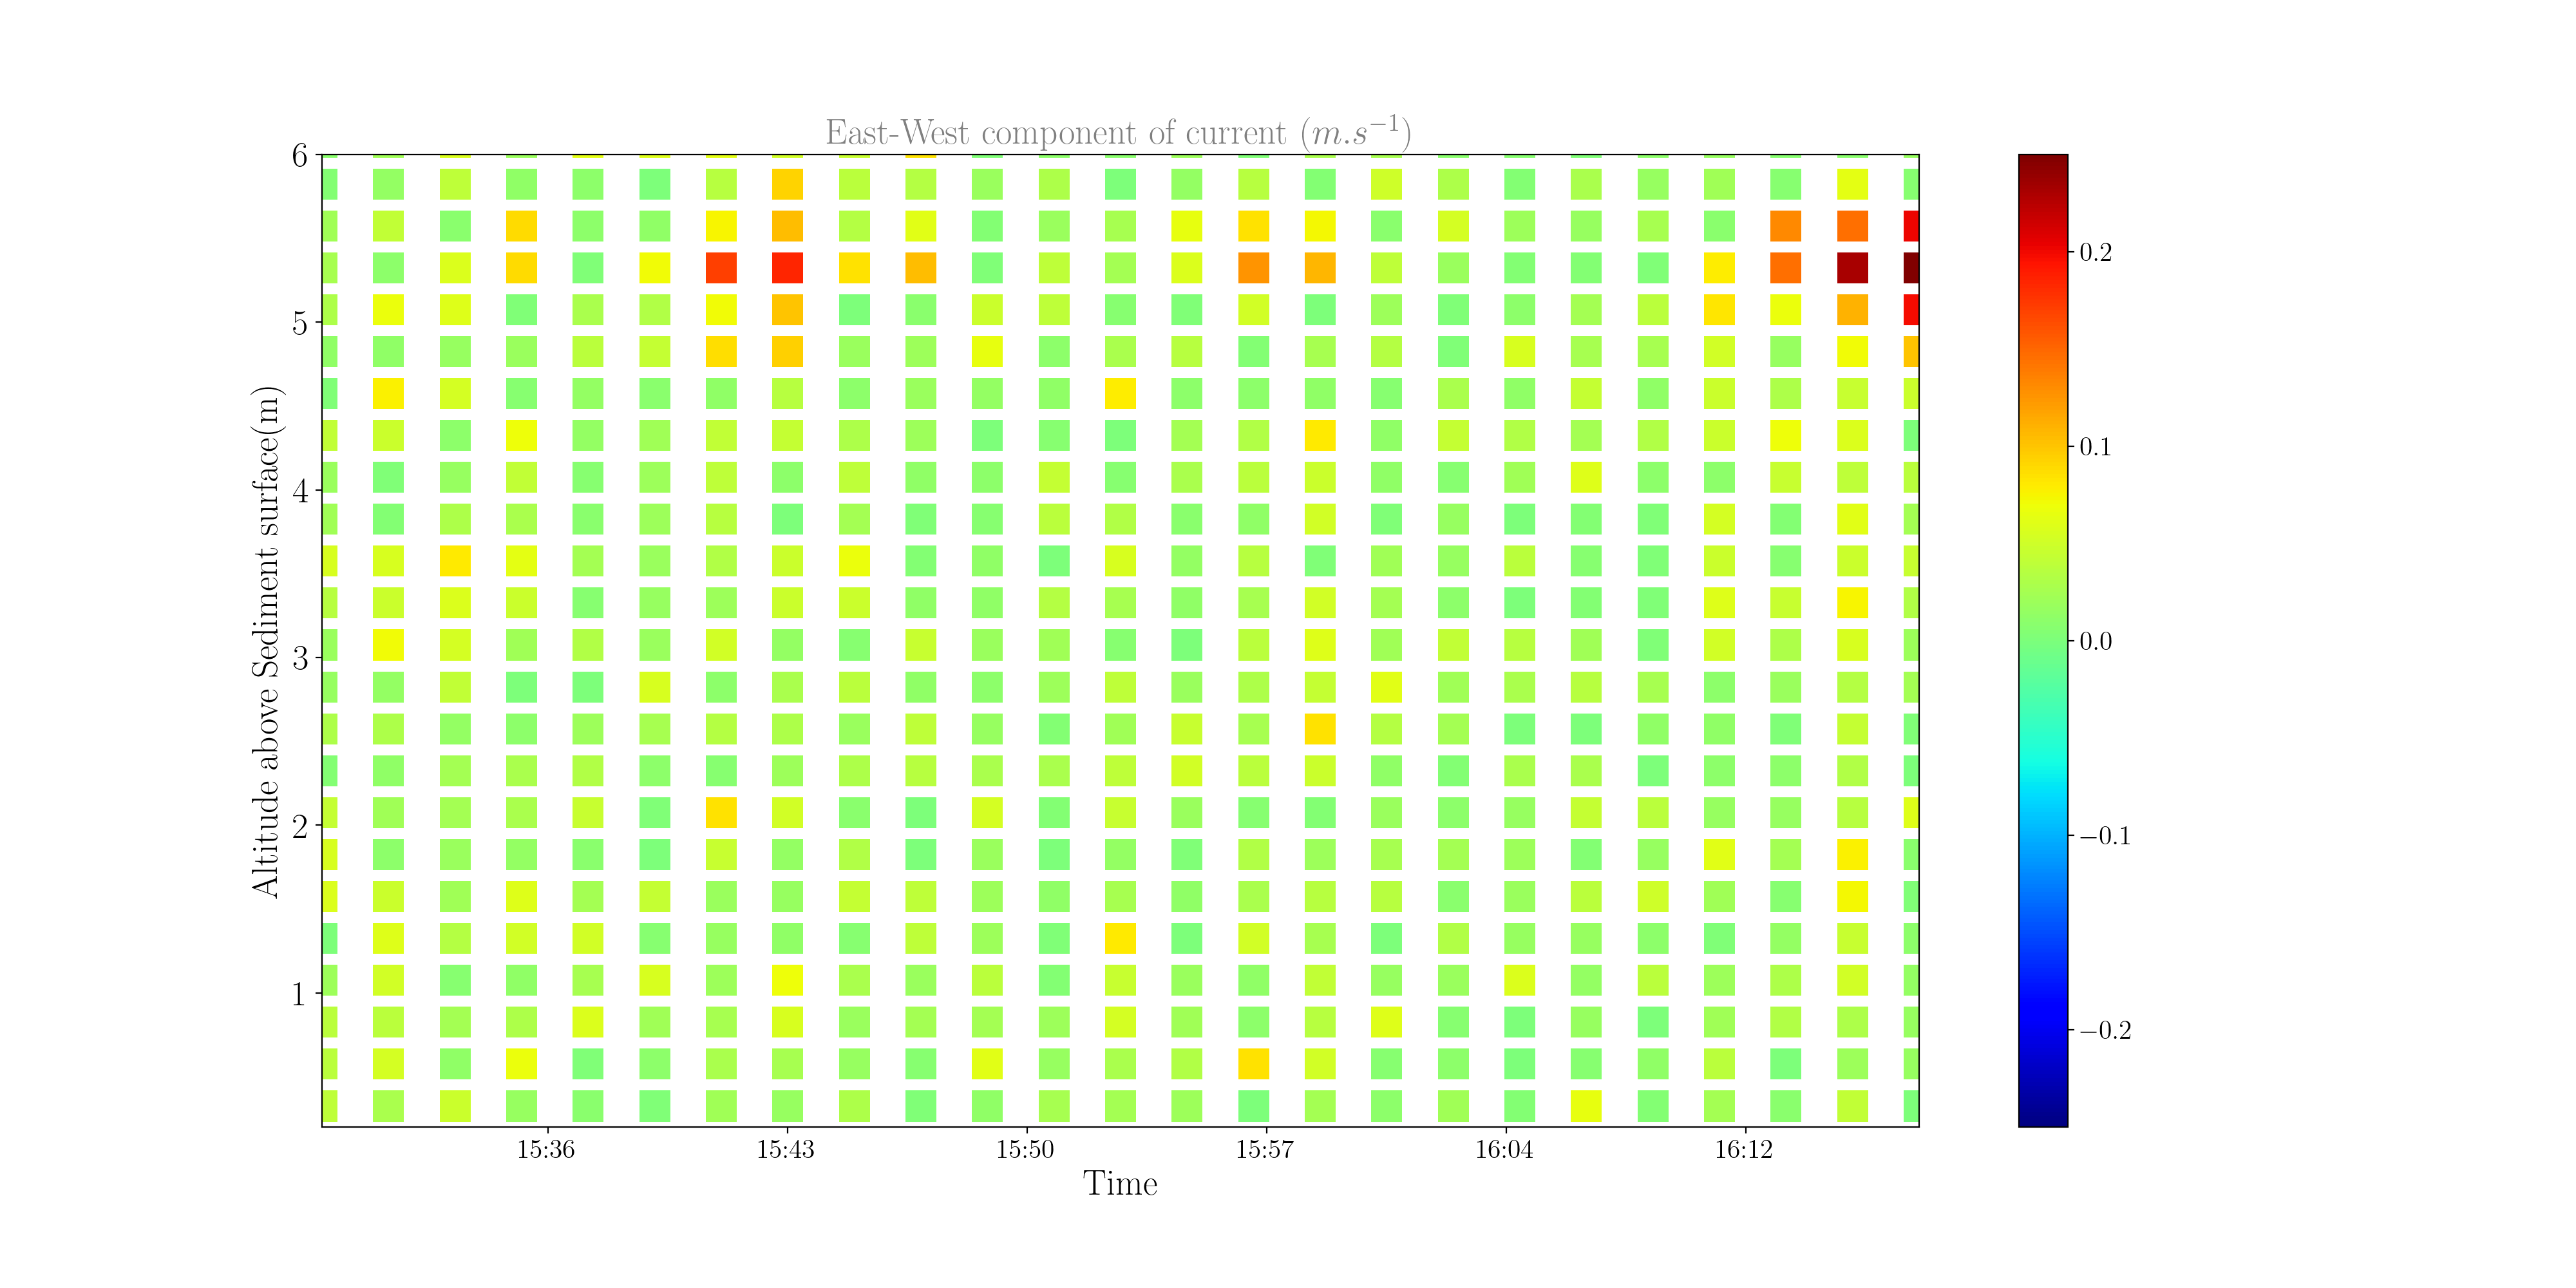
\includegraphics[width=0.8\textwidth]{18032102scatterv1.png}
		\caption{Intensité du courant selon la composante Est-Ouest de 15h30 à 16h20 ($m.s^{-1}$).}
	\end{center}
\end{figure}
L'intensité du courant selon la composante Est-Ouest est comprise entre 0,1 $m.s^{-1}$ et 0,25 $m.s^{-1}$ à la surface pour les quelques points mesurés.\\

\subsection{}
Blabla sur les résultats Aquadopp

\section{SADCP}
\end{document}
